\chapter{Аппаратура для проведения исследований} \label{chapt2}

\section{Прибор Дэпрон}

Прибор Дэпрон разрабатывался как исследовательский инструмент для решения широкого круга научных задач. Основной задачей прибора является измерение мощности дозы и потоков ионизирующих излучений. Дополнительными задачами выделены регистрация нейтронов тепловых энергий и высокоэнергичных частиц. Такое сочетание решаемых задач, для прибора относительно небольшого веса, является уникальным и позволяет надеяться на получение достаточно подробной информации о радиационной обстановке на борту КА. 

\subsection{Устройство прибора}

В состав прибора ДЭПРОН входят два узла с полупроводниковыми детекторами и два узла с газоразрядными гелиевыми счетчиками нейтронов. Также в состав прибора входят узлы усиления и формирования сигналов от полупроводниковых и нейтронных детекторов и узел цифровой обработки сигналов.


Поглощенная доза регистрируется узлами с полупроводниковыми детекторами. Для получения информации о величине поглощенной дозы используется принцип регистрации величины заряда в объеме полупроводника, пропорционального энерговыделению в данном объеме. 

\begin{equation}\label{eq:benghin_doze}
D = \frac{E}{m} = \dfrac{w_i \cdot\dfrac{q}{e}}{m}
\end{equation}
где \begin{description}
	\item[$ D $] поглощенная доза
	\item[$ E $] энергия поглощенная в чувствительном объеме
	\item[$ m $] масса чувствительной зоны детектора
	\item[$ w_i $] энергия формирования np пары
	\item[$ e $] заряд электрона
	\item[$ q $] электрический заряд образованный в чувствительном объеме
\end{description}
Оба полупроводниковых детектора и скомпонованы в кассету и расположены в относительной близости друг от друга. Схема построения прибора с параллельным расположением двух полупроводниковых детекторов была использована для получения информации о ЛПЭ частиц, прошедших одновременно оба детектора. Спектр ЛПЭ зарегистрированных частиц позволяет вычислить эквивалентную дозу, используя постулированный в НРБ-99/2009 \cite{nrb2009} коэффициент качества ионизирующего излучения. Для перехода от поглощенной дозы в кремнии к эквивалентной дозе потребуется пересчет зарегистрированного спектра ЛПЭ в спектр ЛПЭ в воде, который производится умножением на коэффициент $1,21$.
 Функциональная схема прибора ДЭПРОН показана на рисунке \ref{fig:Depron_blocksch}.
 
\begin{figure}
\centering
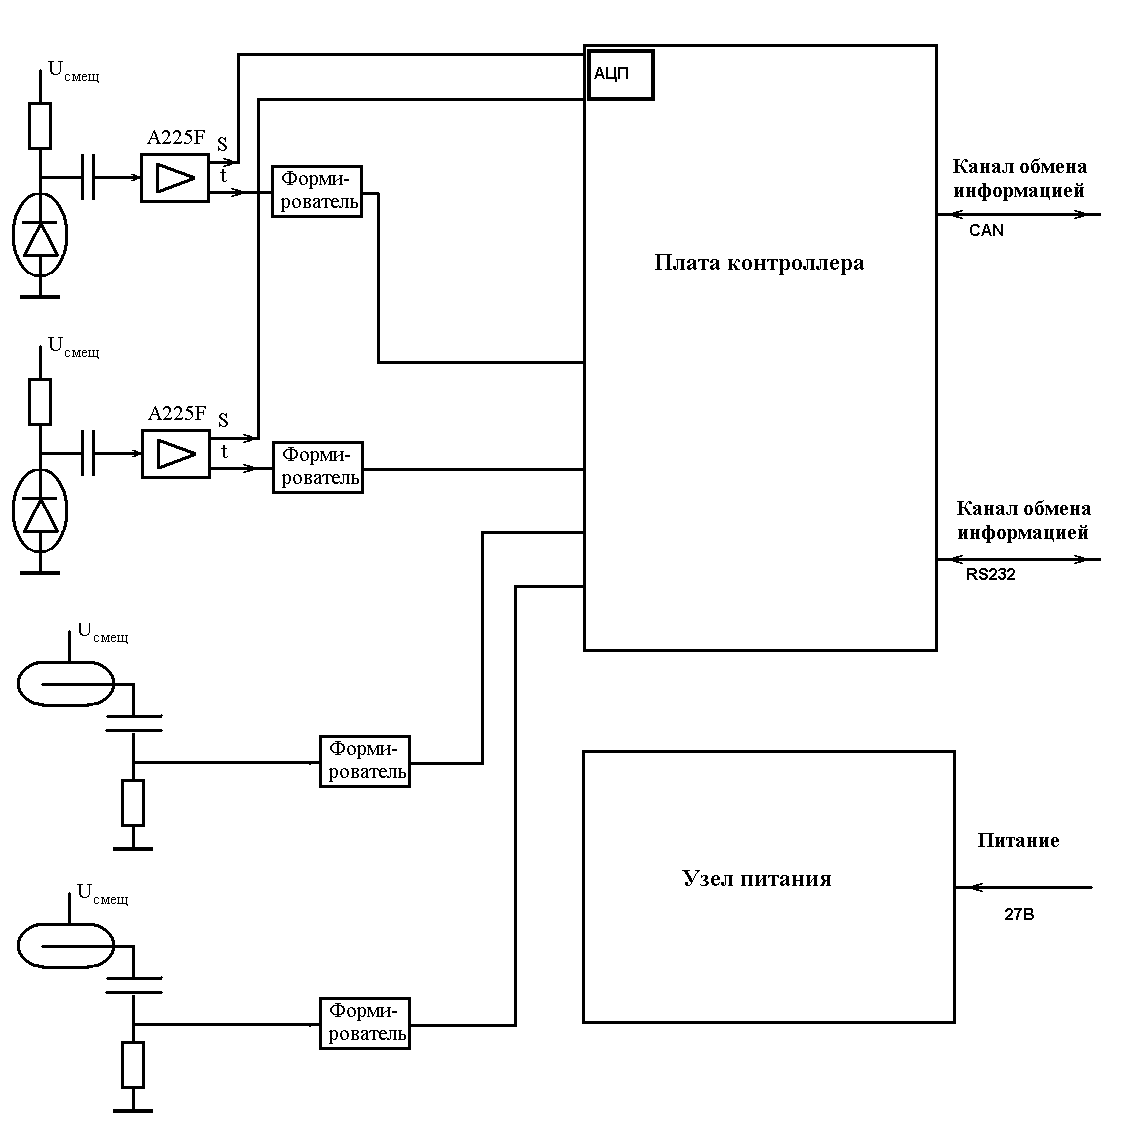
\includegraphics[width=0.8\linewidth]{images/Depron_blocksch}
\caption{Блок-схема прибора ДЭПРОН}
\label{fig:Depron_blocksch}
\end{figure}


%\newpage
%============================================================================================================================
\section{Конструктивные особенности прибора}

Прибор состоит из одного блока, габаритный чертеж которого представлен в Приложении 1. Габаритные размеры прибора: длина  280~мм, ширина 160~мм, высота 78~мм. Масса прибора - 3~кг. Корпус прибора составлен из шести пластин Д16т -- листового дюралюминия, толщиной 4,5~мм, обработанного на станке ЧПУ. В каждой пластине фрезерованы повторяющиеся выборки треугольной формы до толщины 2~мм. Выборки расположены таким образом, чтобы сформировать «ребра» жесткости в стенках прибора, как видно на рисунке \ref{fig:viborki}. С лицевой стороны пластины корпуса оксидированы, с целью получения электропроводной поверхности всего прибора.

\begin{figure}
\centering
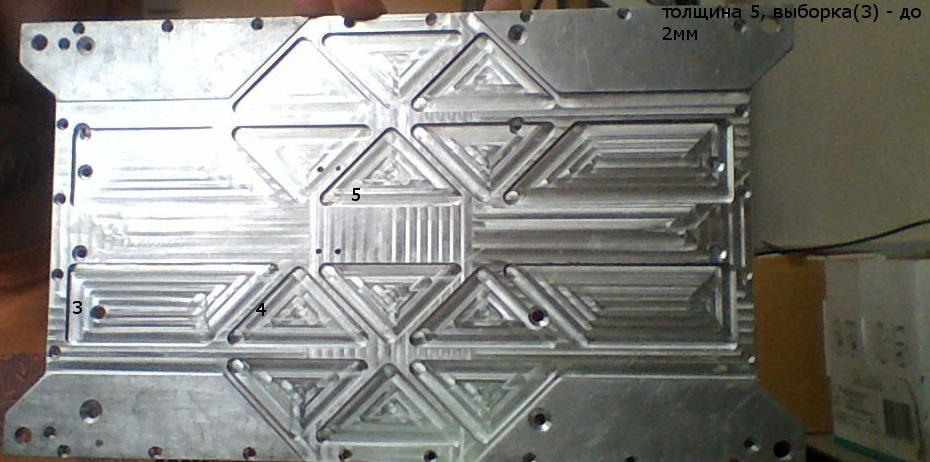
\includegraphics[width=0.7\linewidth]{images/viborki1}
\caption{ Вариант размещения выборок в днище прибора ДЭПРОН.}
\medskip
{\small В последствии данный вариант переработан исходя из конструктивных соображений крепления модулей электроники и улучшения сброса тепла от источников питания, через термо-контакт с бортом КА. }
\label{fig:viborki}
\end{figure}


На лицевом торце прибора расположены два разъема СНП-333, используемых для передачи данных в БИ аппаратуры спутника (разъем Х1) и для передачи питания в прибор ДЭПРОН от бортовой аппаратуры спутника (разъем Х2). Также на лицевой панели находятся два разъема РС-7 предназначенные для передачи информации по каналу RS232 от прибора ИМИСС-1 (разъем Х5) и сквозной передачи питания от бортовой аппаратуры к прибору ИМИСС-1 (разъем Х4). Во всех перечисленных разъемах предусмотрен контроль стыковки разъемов с помощью короткозамкнутых линий, а также дублирование информационных и токонесущих линий.


Дополнительно на лицевую панель прибора вынесен технологический разъем РС 19 ХТ3, используемый для проверки функционирования прибора в лабораторных условиях методом подачи на детекторные узлы калиброванных сигналов с генератора, а также для контроля внутренних рабочих напряжений. Проверка работоспособности прибора и подача сигналов с генератора осуществляется с помощью блока КПА, имеющему четыре экранированных канала для передачи низкоамплитудных сигналов и два светодиодных индикатора для контроля наличия рабочих напряжений  $+5$~В и $  +12$~В в приборе ДЭПРОН.  В штатном режиме работы данный разъем не подключен и закрыт заглушкой. Схема распределения линий в разъемах представлена в Приложении 2.

Платы электроники блоков усиления и формирования аналоговых сигналов располагаются в трех тонкостенных алюминиевых кассетах и выполнены в формате 11-ти контактных печатных плат размерами 34~ммх50~мм (\ref{fig:Depron_inside}). Данный формат печатных плат распространен в производстве научной аппаратуры изготовления НИИЯФ МГУ и с успехом применяется для космической аппаратуры уже на протяжении нескольких десятков лет. Применение данного стандарта позволяет соблюсти принцип модульности построения приборов, используя отработанные в космических условиях надежные схемы, компонуя из них тракты с параметрами, заданными потребностями текущих экспериментальных задач. 

\begin{figure}
\centering
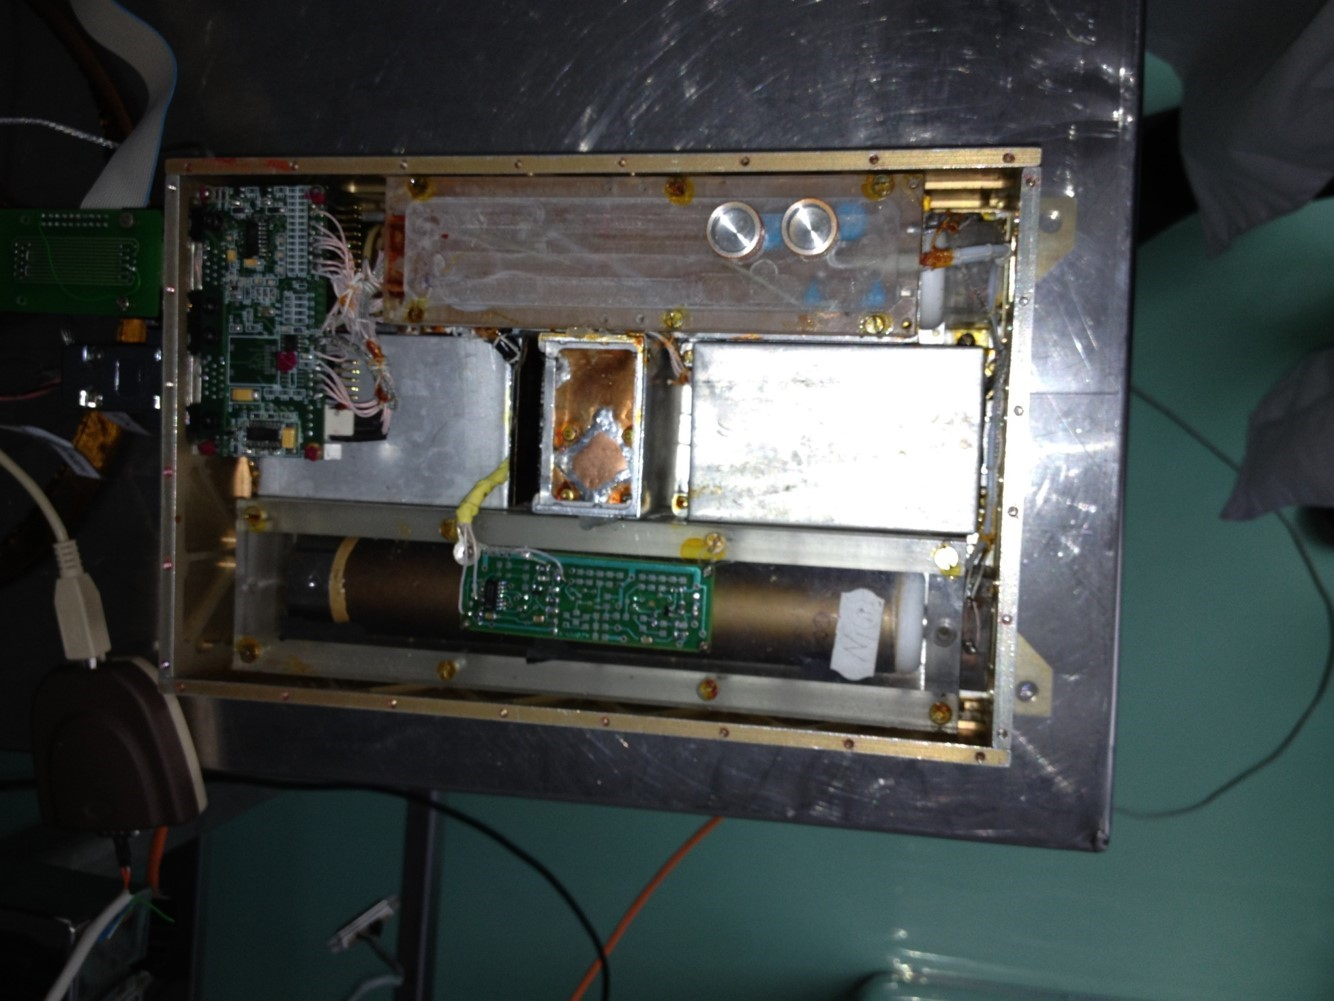
\includegraphics[width=0.7\linewidth]{images/Depron_inside}
\caption{Внутренняя компоновка модулей прибора ДЭПРОН. Вид сверху со снятой крышкой прибора.}
\label{fig:Depron_inside}
\end{figure}


В средней части рисунка последовательно располагаются три корпусных кассеты с платами электроники: левая и правая кассеты содержат платы формирователей триггерных сигналов от детекторов, центральная кассета ориентирована перпендикулярно и содержит две платы полупроводниковых детекторов и ЗЧУ, а также платы дополнительного усиления.

В нижней части рисунка находится нейтронный счетчик СИ13Н (цилиндр), экранированный 1 см оргстекла

\section{Детекторы}

Дозиметр заряженных частиц выполнен на кремниевых ионно-имплантированных Д1 пролетных детекторах, работающих в режиме регистрации амплитуд импульсов. Детекторы изготовлены по специальному заказу НИИЯФ МГУ в ООО «Детектор-СИ» в соответствии с АБЛК.418219.402ТУ. Данные детекторы предназначены для спектрометрии и радиометрии заряженных частиц в составе предназначенной для этих целей аппаратуры. Чувствительный элемент детектора изготовлен из высокоомного кремния n--типа по технологии ионной имплантации. Рекомендуемая схема включения детектора приведена на рисунке \ref{fig:detector_sch}. 


\begin{figure}[h]
	\centering
	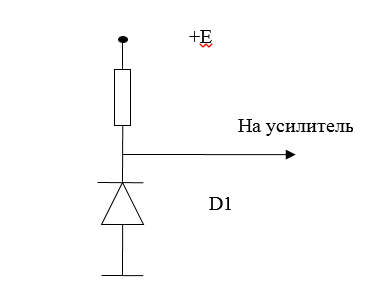
\includegraphics[width=0.5\linewidth]{images/detector_sch}
	\caption{Схема включения детектора.}
	\medskip
	\small
	\begin{description}
		\item[+Еп] источник напряжения;
		\item[Rсм] сопротивление смещения;
		\item[D1] Детектор.
	\end{description}			
	\label{fig:detector_sch}
\end{figure}
	


Детекторы могут эксплуатироваться при атмосферном давлении или в вакууме до 10\textsuperscript{-6} мм.рт.ст., таким образом подходят для размещения  в не герметичном корпусе прибора ДЭПРОН. Подробные значения параметров детекторов приведены в таблице \ref{tab:detectors}.

\begin{table} 

	\begin{tabular}{p{10cm}|cc}
		Наименование параметра                                       & Фактические параметры &  \\ \hline
		Рабочее напряжение, В                                        &          90           &  \\
		Обратный ток, нА                                             &           4           &  \\
		Энергетический эквивалент шума, кэВ                          &           5           &  \\
		Постоянная времени квази-гауссова формирования импульса, мкс &           2           &  \\
		Предельно допустимое напряжение, В                           &          130          &  \\
		\multicolumn{2}{l}{Примечания: Аттестация производилась при 26 C.}                   &
	\end{tabular} 
	\caption{Полупроводниковые детекторы прибора ДЭПРОН (по материалам ТУ)}
		\label{tab:detectors}
\end{table}



\subsection{Телескоп детекторов}
В приборе ДЭПРОН используются два полупроводниковых детектора. Детекторы образуют телескоп, то есть расположены параллельно на определенном расстоянии, что обеспечивает возможность регистрировать спектр ионизационных потерь.
Дополнительно использование двух детекторов позволяет повысить уровень надежности всего регистрирующего тракта.

Схематично относительное расположение детекторов показано на рисунке~\ref{fig:telescope}.  Расстояние между детекторами выбрано 18 мм, таким образом, что телесный угол полета частиц, проходящих через оба детектора оказывается около 30 градусов. 


%\begin{tikzpicture}
%\draw[dashed,color=gray] (0,0) arc (-90:90:0.5 and 1.5);% right half of the left ellipse
%\draw[semithick] (0,0) -- (4,1);% bottom line
%\draw[semithick] (0,3) -- (4,2);% top line
%\draw[semithick] (0,0) arc (270:90:0.5 and 1.5);% left half of the left ellipse
%\draw[semithick] (4,1.5) ellipse (0.166 and 0.5);% right ellipse
%\draw (-1,1.5) node {$\varnothing d_1$};
%\draw (3.3,1.5) node {$\varnothing d_2$};
%\draw[|-,semithick] (0,-0.5) -- (4,-0.5);
%\draw[|->,semithick] (4,-0.5) -- (4.5,-0.5);
%\draw (0,-1) node {$x=0$};
%\draw (4,-1) node {$x=l$};
%\end{tikzpicture}



\begin{figure}	
	\centering
	\begin{tikzpicture}[scale=2, transform shape]
	\pic [fill=magenta, text=blue, draw=blue] at (5,0) {annotated cuboid={width=10, height=0.3, depth=10, units=мм}};
	\pic [fill=green, text=green!50!black, draw=green!25!black] at (5,-1.8) {annotated cuboid={width=10, height=0.3, depth=10, units=мм}};
	
	\draw[|->,semithick] (7,-1.8) -- (7,0);
	\draw (8,-1.8) node {$z=0$};
	\draw (8,0) node {$z=18$};
	%	\pic at (1,-3) {annotated cuboid={width=150, height=200, depth=250, scale=.01, units=m}};
	%	\pic [fill=cyan, text=blue!75!cyan, draw=blue!75!cyan] at (-3,-2) {annotated cuboid={width=15, height=18, depth=13.5, units=}};
	\end{tikzpicture}
	\caption{Телескоп детекторов прибора ДЭПРОН, масштаб 1:2}
	\label{fig:telescope}
\end{figure}

\subsubsection{Расчет геометрического фактора телескопа}
В соответствии с работой \cite{Thomas1972} общий геометрический фактор можно вычислить исходя из соображений затенения одного детектора вторым, что для геометрии с прямоугольными детекторами дает:

\[ G = Z^2 \int_{-X_1}^{X_1} \int_{-Y_1}^{Y_1} 
			\int_{-X_2}^{X_2} \int_{-Y_2}^{Y_2}
			\frac{dx_1dy_1dx_2dy_2}{\left\lbrace Z^2 + (x_2-x_1)^2 + (y_2-y_1)^2\right\rbrace^2 }\]

Численный расчет в пакете Mathcad ( рисунок \ref{fig:mathcadGeomfactor}) дает в результате для нашего случая геометрический фактор 0.145,  так как геометрический фактор отдельного детектора равен $ 4\pi $ и мы имеем два идентичных детектора, поэтому удваиваем результат интегрирования. Поправочный коэффициент для энерговыделения в телескопе детекторов 0,043, он рассчитан по соотношению \ref{eq:lpe_koef}, где $ S_0 $ площадь чувствительной поверхности.
\begin{equation}\label{eq:lpe_koef}
 \xi = \frac{Z}{2 \pi S_0 } \cdot \int_{-X_1}^{X_1} \int_{-Y_1}^{Y_1} 
\int_{-X_2}^{X_2} \int_{-Y_2}^{Y_2}
\frac{dx_1dy_1dx_2dy_2}{\left\lbrace Z^2 + (x_2-x_1)^2 + (y_2-y_1)^2\right\rbrace^2 }^{\frac{3}{2}}
\end{equation}




\begin{figure}[h!]
\centering
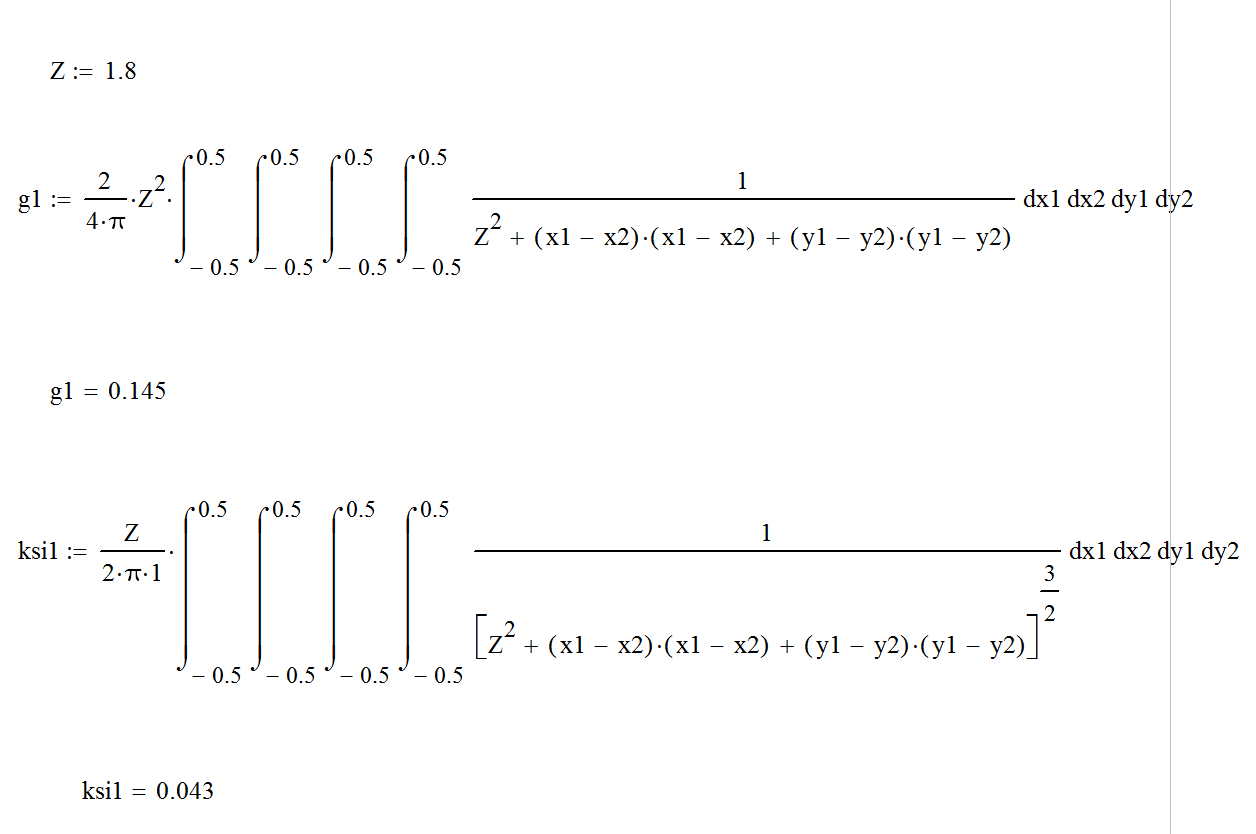
\includegraphics[width=0.7\linewidth]{images/mathcadGeomfactor1}
\caption{ Расчет геометрического фактора телескопа в системе Mathcad}
\label{fig:mathcadGeomfactor}
\end{figure}

%\begin{figure}
%\centering
%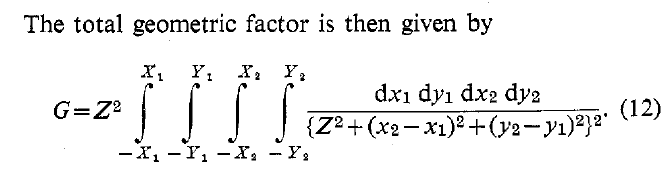
\includegraphics[width=0.7\linewidth]{images/totalgeomfactorintegral}
%\caption{}
%\label{fig:totalgeomfactorintegral}
%\end{figure}

%\begin{figure}
%\centering
%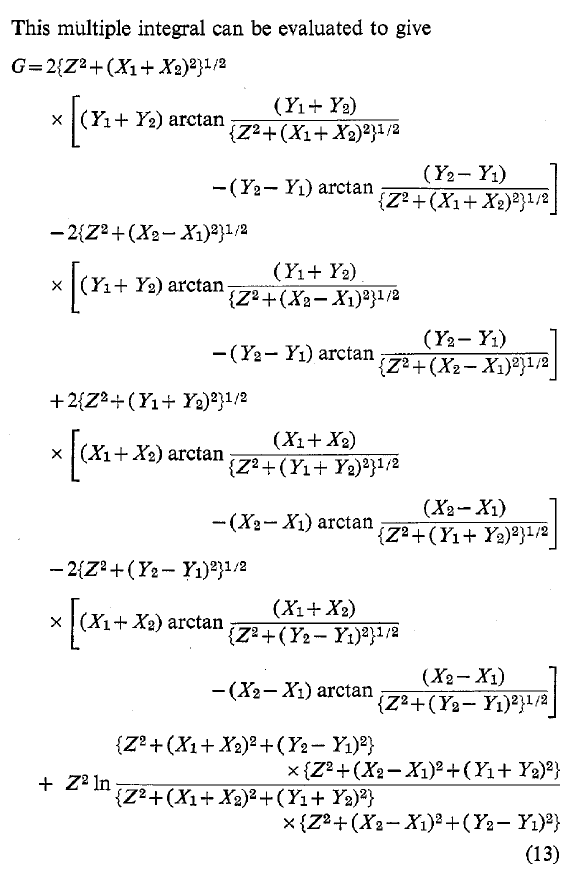
\includegraphics[width=0.7\linewidth]{images/totalgeomfactorsolved}
%\caption{}
%\label{fig:totalgeomfactorsolved}
%\end{figure}
%\begin{figure}
%\centering
%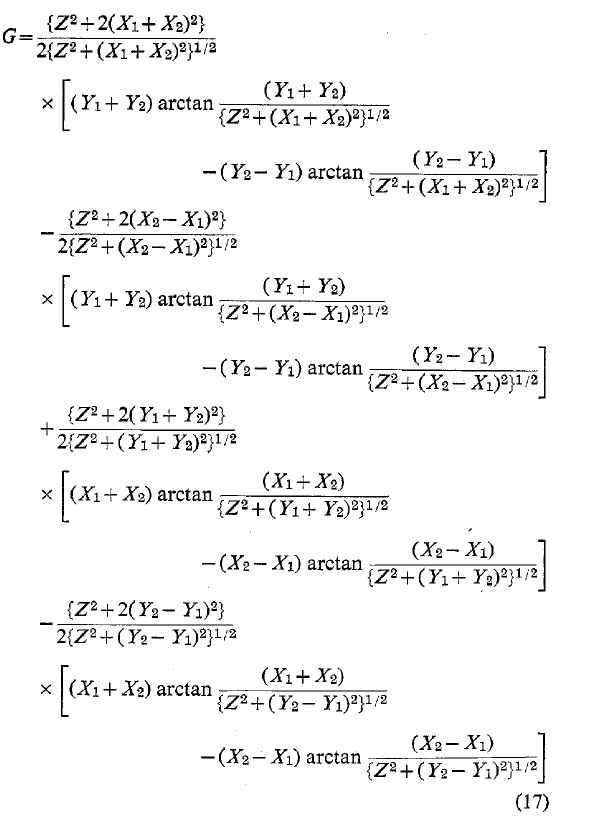
\includegraphics[width=0.7\linewidth]{images/totalgeomfactorsolved2}
%\caption[для интенсивности]{}
%\caption{}
%\label{fig:totalgeomfactorsolved2}
%\end{figure}



\subsection{Нейтронные детекторы}

Детектор нейтронов выполнен на счётчике медленных нейтронов «СИ-13Н», представляющем собой газоразрядный счетчик, работающий в режиме коронного разряда. Для обеспечения надежности используются 2 счетчика. Второй детектор нейтронов окружен замедляющей оболочной из поликарбоната, что позволило расширить энергетический диапазон регистрируемых нейтронов. При прохождении нейтрона через газ Не-3, наполняющий счетчик, происходит ядерная реакция:
\[ n+^3\!He = p+T+764 \textrm{ кэВ}\]
При этом энергия между тритоном и протоном может распределяться в различных соотношениях, а наиболее вероятно распределение в соответствии с массами продуктов 1:3.
%\begin{figure}
%\centering
%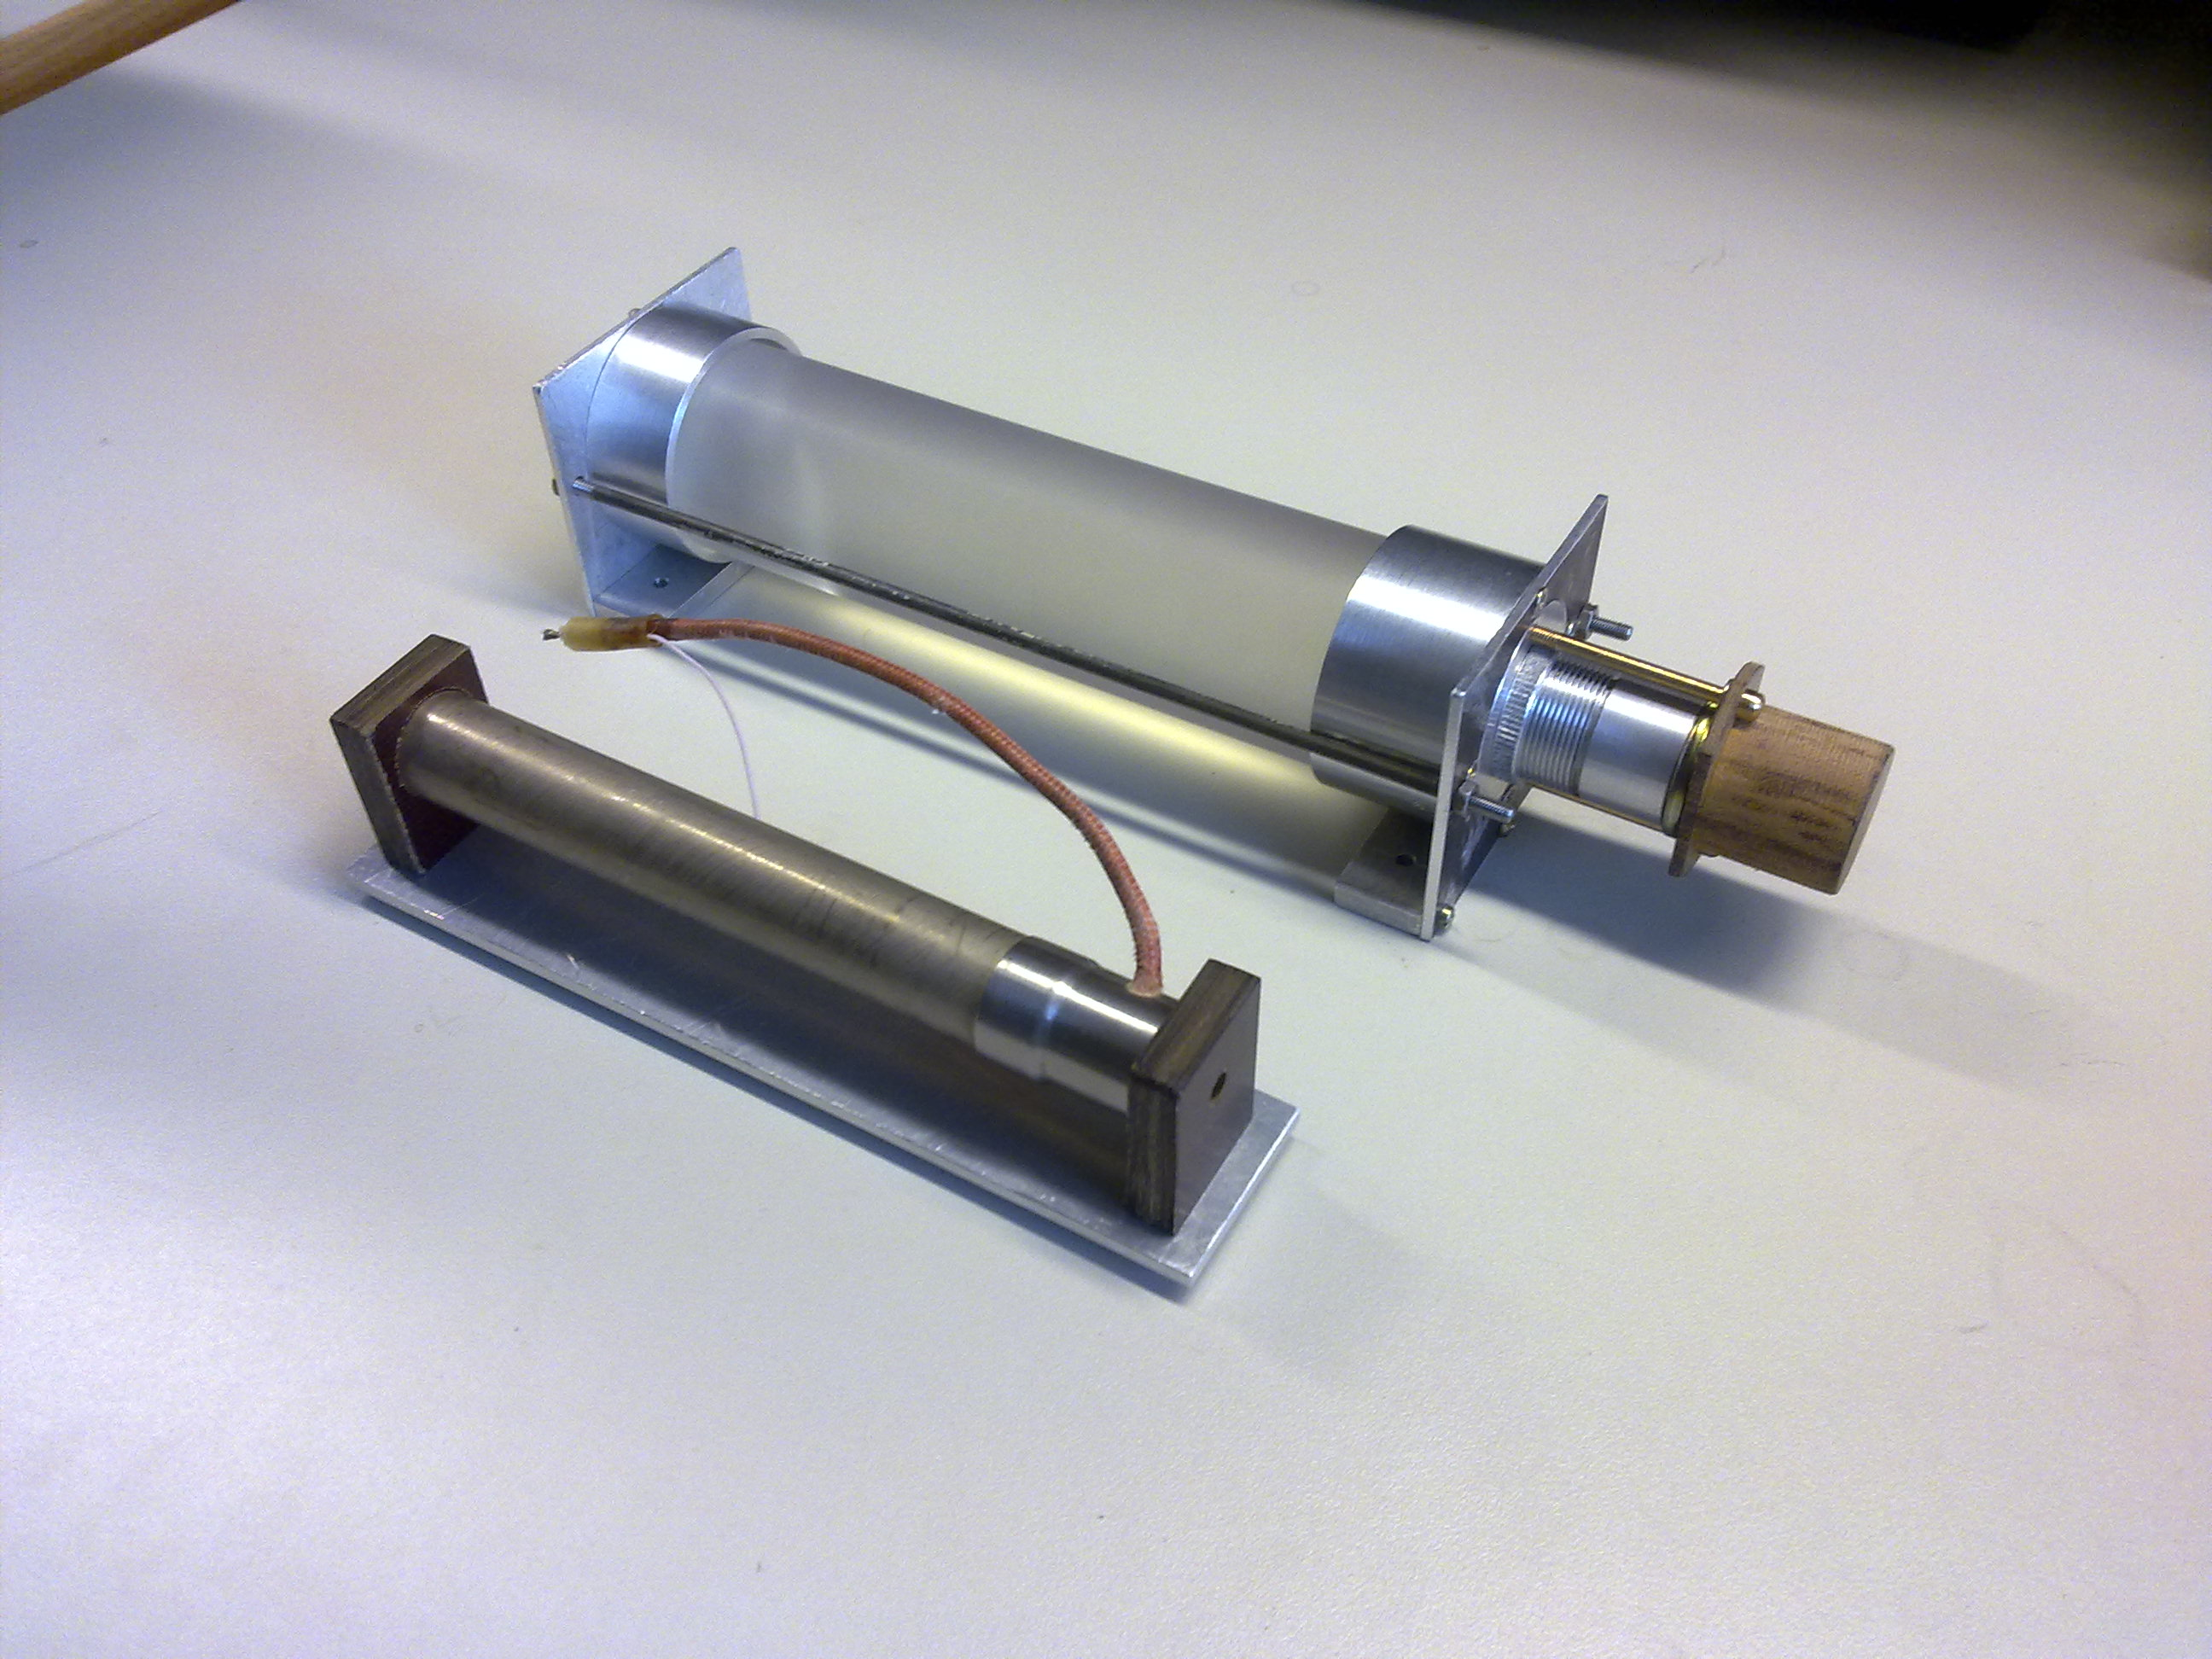
\includegraphics[width=0.7\linewidth]{images/04062010072}
%\caption{Гелиевый счетчик нейтронов и кожух из органического стекла внутрь которого помещается второй счетчик нейтронов.}
%\label{fig:04062010072}
%\end{figure}


Продукты реакции вызывают ионизацию газа в счётчике, что приводит к образованию газового разряда и появлению электрического импульса на электроде счетчика. Импульс поступает на вход усилителя-формирователя и, затем, поступает на регистр прерываний процессора, где используется для подсчета числа зарегистрированных нейтронов.
\cite{Shavrin2002}

В материалах препринта \cite{Shavrin1990} сделан вывод о чувствительности $ \eta $ и геометрическом факторе счетчиков нейтронов: 
\begin{equation}\label{eq:sens}
 \eta = \frac{N}{n} 
\end{equation}

где $ N $ счет в детекторе, а $ n $ исходный поток нейтронов. Чувствительность счетчиков зависит от энергии нейтронов и конфигурации прибора. Так как толщина материала стенок прибора незначительна по сравнению с пробегом нейтронов в алюминии, мы можем считать, что счетчики нейтронов не имеют четко выраженных пиков на диаграмме направленности.

Для полного описания работы нейтронный счетчиков необходимо учитывать вероятность регистрации заряженных частиц и гамма-излучения, а также собственную радиоактивность счетчиков (0.083имп/c). Для прибора Дэпрон собственный фон счетчиков незначителен по сравнению со средним уровнем счета на орбите. 

%\newpage
%============================================================================================================================
\section{Аналоговая обработка сигналов}

Платы полупроводниковых детекторов и предусилителей (внутренний номер SSD006) изготовлены методом фотолитографии в стандартном формате 34х50, использование современных миниатюрных электронных компонент позволило совместить блоки предусиления и детектирования на одной плате и закрыть единым экраном от электромагнитных помех.

Сигнал с полупроводникового детектора поступает на зарядочувствительный предусилитель A225F \ref{fig:a225}, фирмы AMPTEC, специализирующейся на производстве компонент для космической промышленности. 


\begin{figure}
\centering
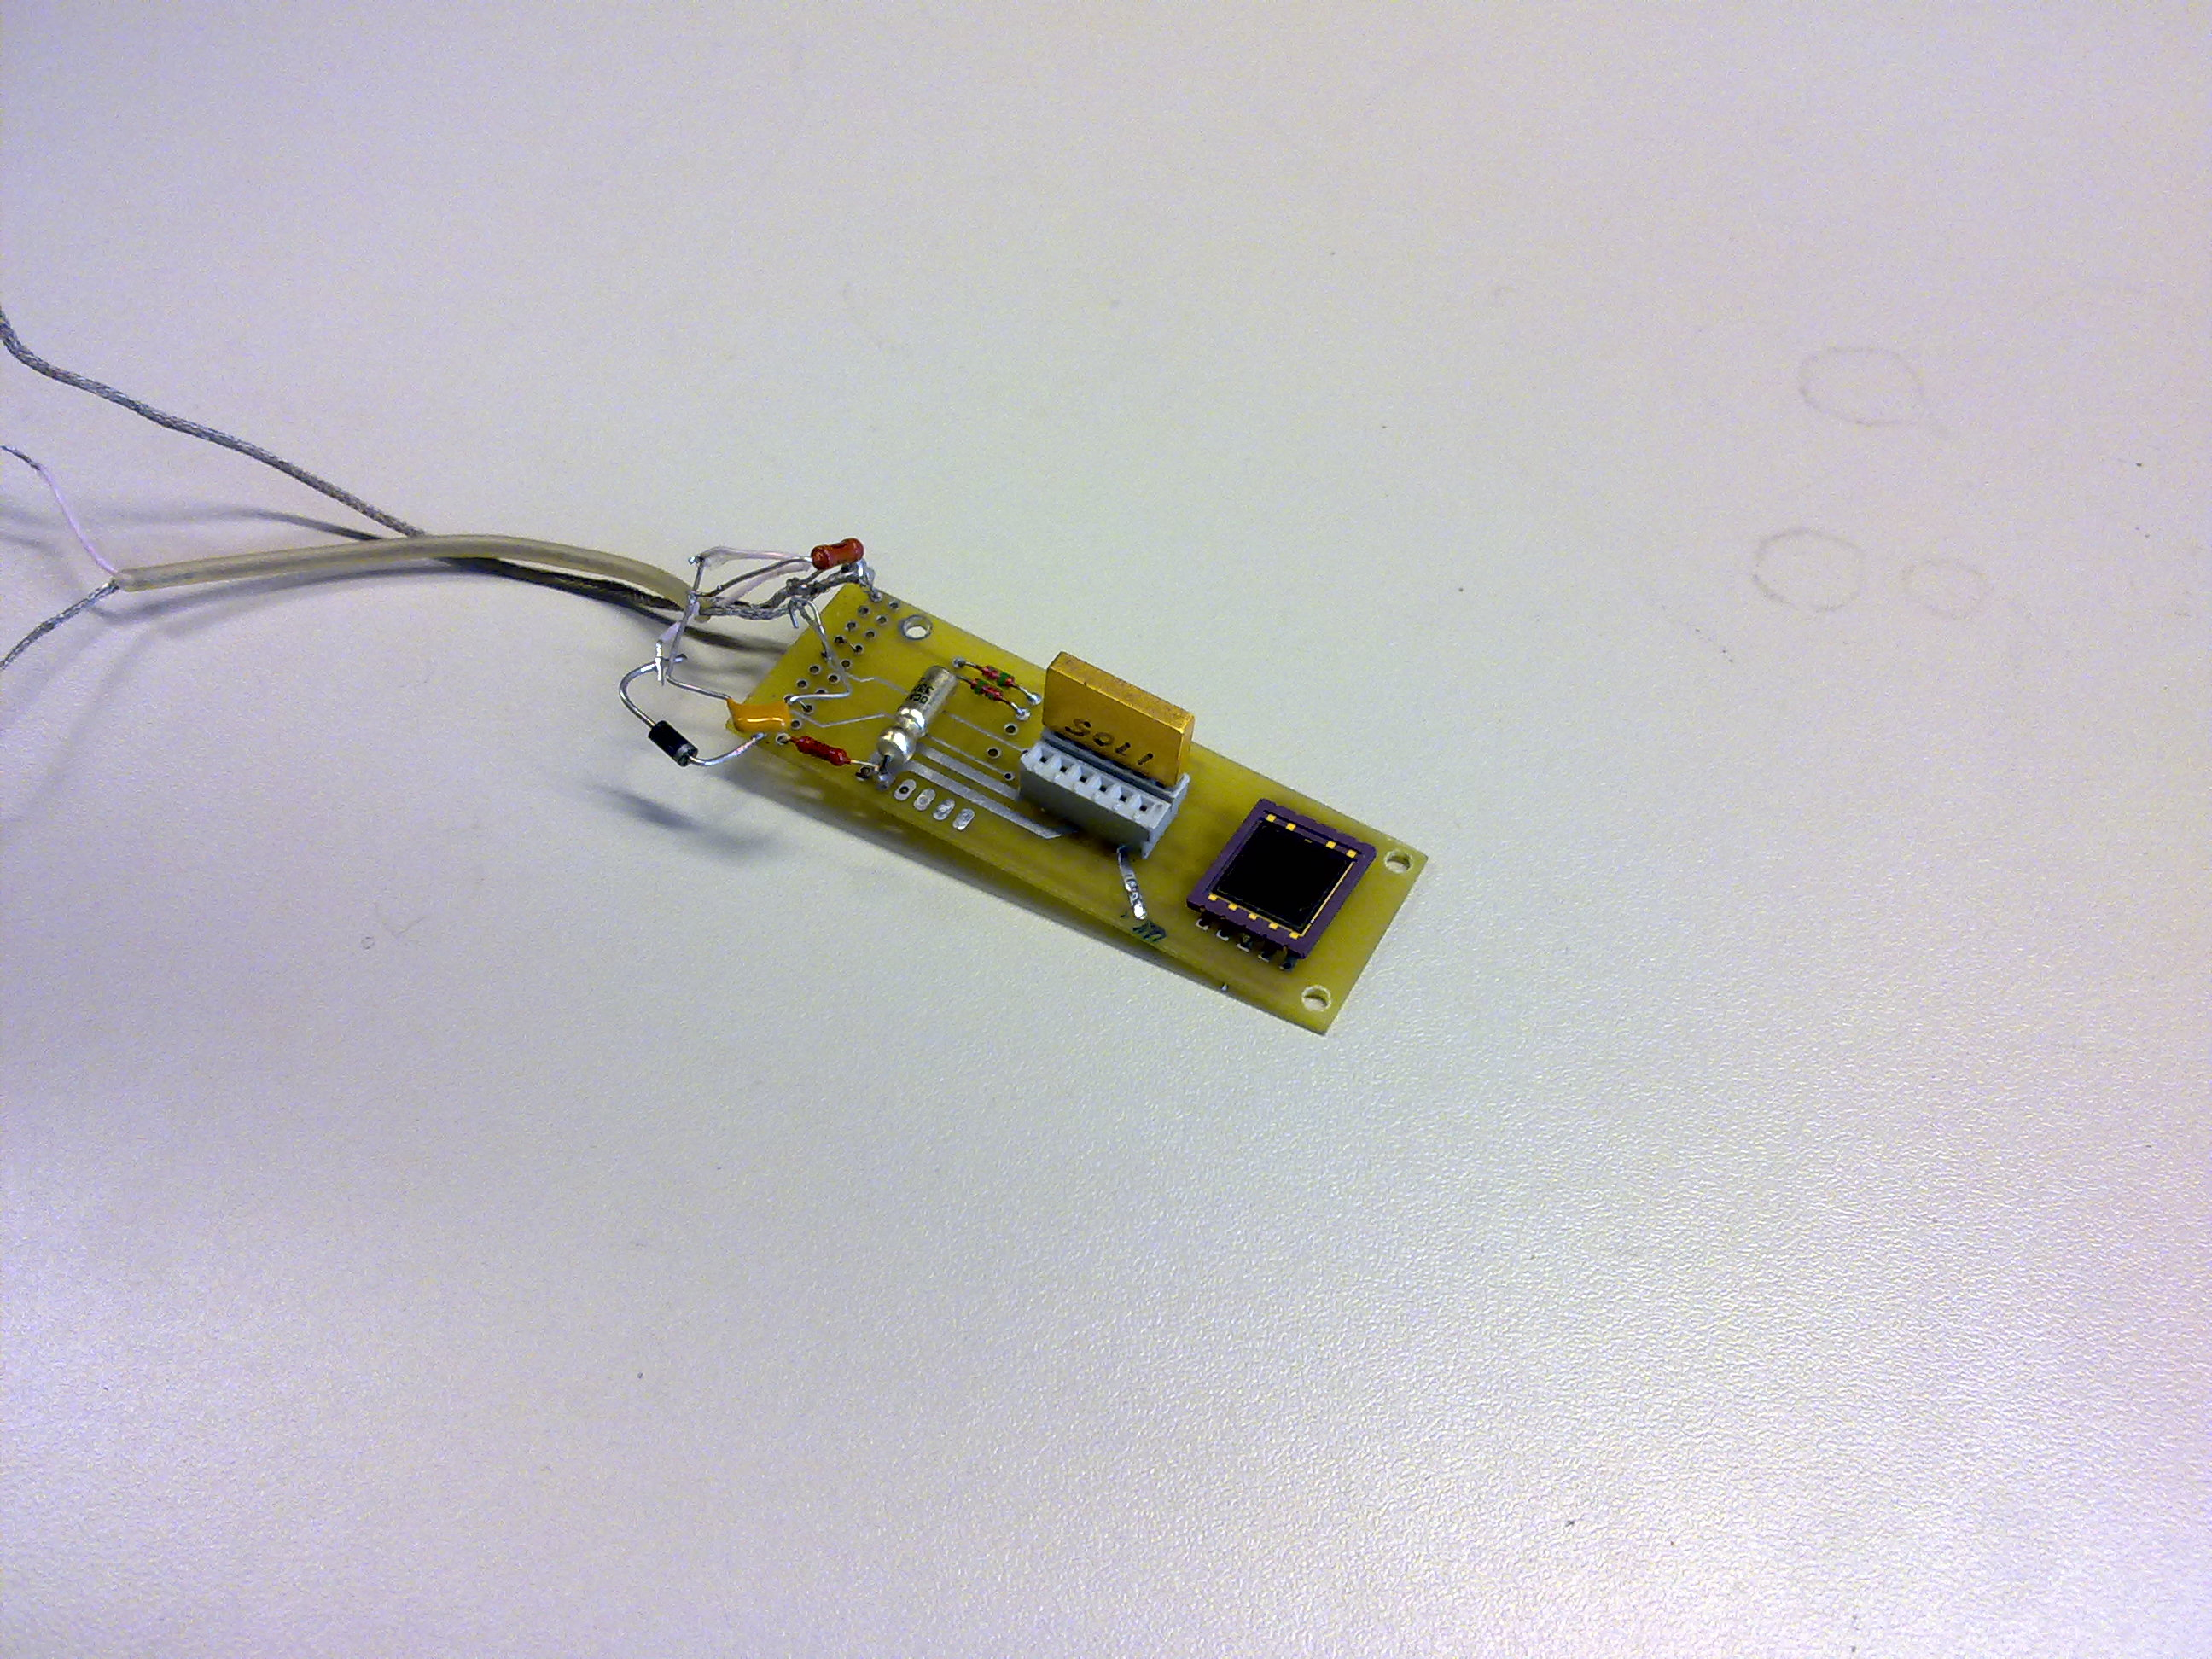
\includegraphics[width=0.7\linewidth]{images/04062010073}
\caption{Фотография прототипа модуля полупроводникового детектора-предусилителя (A225F)}
\label{fig:a225}
\end{figure}

На выходах предусилителя формируются два сигнала. Один (S-сигнал) - имеет амплитуду пропорциональную заряду, образовавшемуся в детекторе и длительность порядка 5 -- 10~мксек. Этот сигнал поступает на амплитудно-цифровой преобразователь (АЦП). Второй сигнал предусилителя A225F (t-сигнал) имеет короткое, менее 0.5 мксек, время задержки от момента прихода сигнала с детектора до максимума амплитуды и используется для запуска процесса цифровой обработки пришедшего импульса. Этот (t-сигнал) сигнал поступает на вход усилителя и, после усиления, поступает на регистр прерываний процессора, где используется для запуска процесса преобразования амплитуды сигнала, поступившего на АЦП, в код. Дальнейшая обработка сигналов с полупроводниковых детекторов производится микропроцессором прибора в цифровой форме.

%\newpage
%============================================================================================================================
\section{Цифровая обработка сигналов}

Для записи результатов измерений прибора используется внутренняя память микроконтроллера, входящего в состав узла цифровой обработки сигналов. В нее записываются, а затем передаются в Блок Информации КА «Ломоносов» кадры информации.
\begin{figure}
\centering
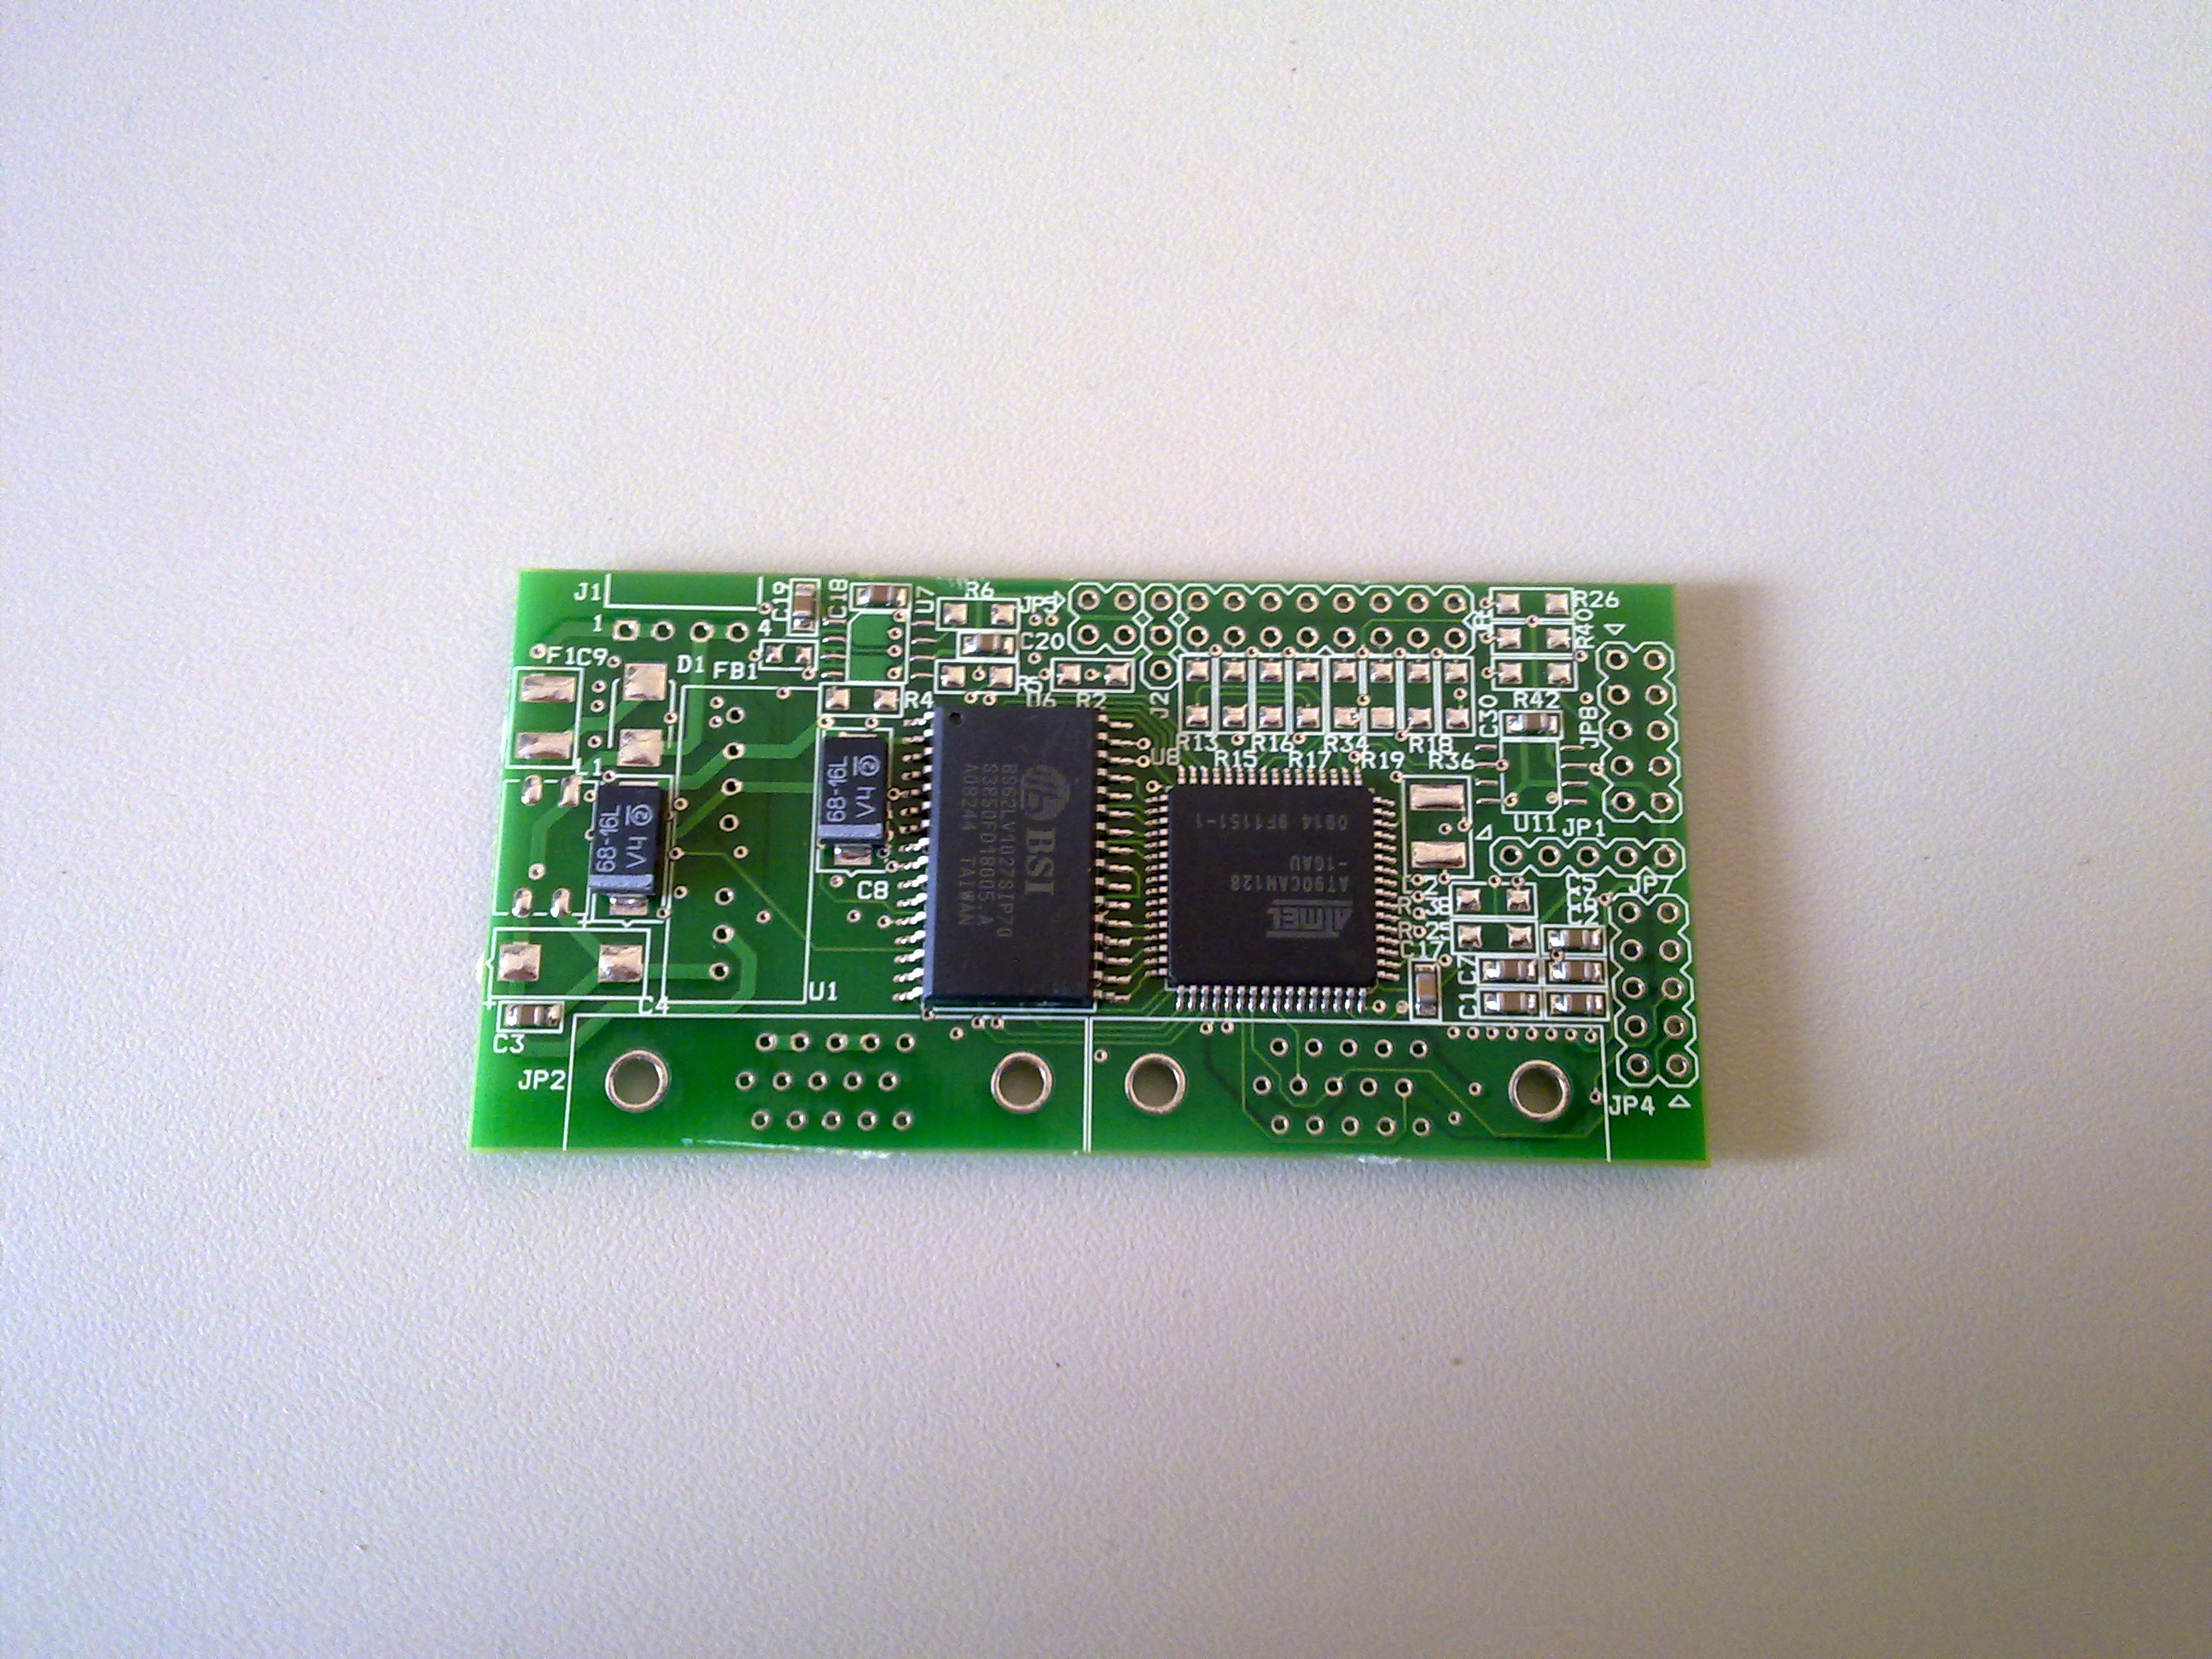
\includegraphics[width=0.7\linewidth]{images/04062010070.jpg}
\caption{}
\label{fig:04062010070}
\end{figure}

На этапе опытно-конструкторских разработок (при макетировании прибора ДЭПРОН) в качестве узла цифровой обработки сигнала использовался 8-битный микроконтроллер ATmega128. Данная микросхема отличается низкой потребляемой мощностью и обладает развитыми средствами ввода данных и обмена информацией, а также достаточной вычислительной мощностью. Печатная плата контроллера была разработана в НИИЯФ МГУ Н.Н. Веденькиным и Д.Г. Аксельродом. На плате расположены два АЦП, а также дополнительная память, независимый преобразователь питания и контроллер обеспечения связи по последовательному каналу (RS232). Как показали опытно-конструкторские работы, проведенные с макетом дозиметра ДЭПРОН, данный узел обеспечивает потребности по бортовой обработке сигналов от детектора по производительности, несмотря на то, что по современным меркам частота работы ядра процессора невелика - 16~МГц. Также выбранный контроллер обладает достаточным для поставленной задачи количеством входных каналов.

Для преобразования амплитуды импульсов, сформированных на выходе аналоговых трактов усиления, использовались 12-ти битные АЦП AD7495 фирмы Analog Devices со скоростью работы 1 MSPS (миллион измерений в секунду). Данные АЦП используют высокоскоростной последовательный интерфейс (SPI -- Serial Peripheral Interface), который был реализован программным способом. Управление моментом захвата амплитуды входного сигнала также производилось программным способом подачей цифрового сигнала «0» на линию CS. 
\begin{figure}
	\centering
	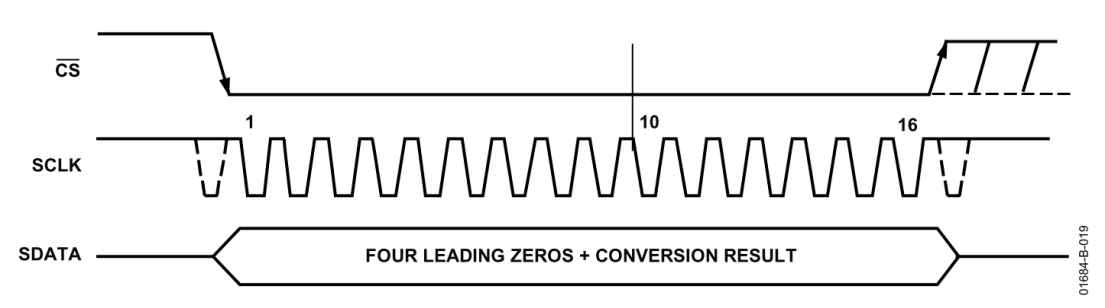
\includegraphics[width=0.7\linewidth]{images/adc}
	\caption{Тактирование использованного в приборе ДЭПРОН режим работы АЦП (AD7495), по материалам \cite{AnalogDevices2005} }
	\label{fig:adc}
\end{figure}

В первой версии платы цифровой обработки сигналов подключение обоих АЦП к контроллеру прибора производилось по независимым каналам: CS (Chip Select -- Активный логический вход АЦП), SCLK (Serial Clock -- логический вход АЦП), SDATA (Data Output -- логический выход АЦП). Задача максимально быстрого захвата сигналов с выхода предусилителя решалась включением встроенного в АЦП устройства выборки и хранения (англ. ``track and hold circuit'') в момент получения контроллером сигнала от таймингового выхода предусилителя. Для этого прерывания контроллера настроены при получении такого сигнала на выдачу управляющего сигнала на вход CS АЦП, ответственного за оцифровку сработавшего канала аналоговой части прибора. Дальнейшая оцифровка амплитуды захваченного в буфере АЦП сигнала производилась после выхода из процедуры обработки прерывания, так как этот процесс отнимает значительное время. Испытания процедуры управления оцифровкой АЦП показали, что точность измерений АЦП чувствительна к временной регулярности тактирующего сигнала, подаваемого на SCLK АЦП. Одной из причин таких нерегулярностей является возможность срабатывания прерывания в ПО контроллера во время исполнения процедуры генерации тактирующих импульсов, что в условиях эксплуатации прибора при высоких потоках ионизирующих излучений (например, в области ЮАА) не редкость. Временное отключение обработки прерываний может устранить данный недостаток работы прибора, однако испытания такого режима работа показали накопление необработанных прерываний в буфере контроллера, которые впоследствии обрабатывались неверно, из-за чего решено отказаться от использования этого режима.

\begin{figure}
\centering
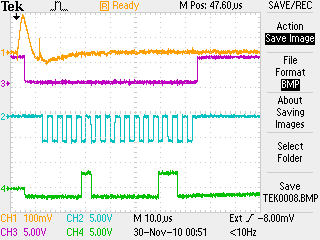
\includegraphics[width=0.7\linewidth]{images/TEK0008}
\caption{Осциллограмма: регулярность тактирующего сигнала, подающегося на SCLK АЦП.}
\label{fig:oscadc}
\end{figure}


Выявление нерегулярности тактирующего сигнала потребовало проверку этого сигнала с помощью осциллографа, снимок экрана представлен на рисунке \ref{fig:oscadc}. Дизассемблирование скомпилированного кода программы микроконтроллера показало критические места кода, требующие изменения алгоритма генерации тактирующих импульсов и добавления промежутков простоя процессора (\texttt{\_nop} -- в коде ``no operation''). Окончательная проверка регулярности сигнала, генерируемого выверенным кодом, производилась снятием временной развертки тактирующего сигнала  на осциллографе. Данный подход использовался и при последующих проверках режимов работы АЦП прибора ДЭПРОН.

%\todo{Рисунок Блок схема подключения АЦП к контроллеру версия 1.}

Таким образом, в первой версии платы цифровой обработки сигналов использовались шесть независимых каналов контроллера, что ограничивало возможность подключения дополнительных информационных каналов с детекторной части прибора. Также одой из проблем данного подхода является двойная нагрузка на микроконтроллер прибора ДЭПРОН, так как управляющие сигналы генерируются программным способом. Такой подход предоставлял сомнительное преимущество в независимом управлении АЦП из программного обеспечения микроконтроллера, поэтому было принято решение изменения способа подключения АЦП.

Следующим конструктивным решением было включение обоих АЦП в параллельный режим работы, когда управляющий (CS) и тактирующий (SCLK) сигналы подаются на оба АЦП. Каналы данных (SDATA) подключены к независимым входам контроллера. 

%\todo{Рисунок Блок схема подключения АЦП к контроллеру версия 2.}

При проектировании Блоков обработки Информации (БИ) было принято решение по организации обмена по каналу CAN между дочерними приборами, входящими в Комплекс Научной Аппаратуры (КНА) «Ломоносов». Однако использованный для макетирования контроллер ATmega128, и данный контроллер был заменен на AT90CAN128. Данное решение было продиктовано минимальными изменениями уже разработанного программного обеспечения и незначительными доработками печатных плат, необходимым для внедрения контроллера AT90CAN128.

Опыт работы с данным контроллером также показал его применимость для целей построения полноценного дозиметра ионизирующих излучений. Тем не менее, по требованию других участников проекта данный контроллер был заменен более современным и более производительным контроллером AT91SAM7X256. Всего в составе КНА насчитывается 4 прибора, в которых использована схема цифровой обработки сигнала на базе AT91SAM7X, некоторые из этих приборов испытывали нехватку производительности данного модуля до замены ЦПУ. В целях унификации разработанный аппаратуры модуль цифровой обработки сигналов и связи был заменен и в приборе ДЭПРОН. Данное изменение состава прибора повлекло за собой необходимость повторения цикла разработки программно-математического обеспечения прибора и проведения повторных калибровок АЦП и счетных каналов схемы цифровой обработки. Необходимость данных работ обусловлена принципиальным отличием архитектуры контроллера: в исходном варианте это архитектура AVR, а в окончательном ARM. 

В финальном варианте цифровая обработка сигналов осуществляется с помощью микропроцессора AT91SAM7X512. Программно-математическое обеспечение ДЭПРОН функционирует на одной микропроцессорной плате SSD234. Данная плата собрана на базе микроконтроллера AT91SAM7X512 производства фирмы ATMEL, и содержит процессор ARM7 TDMI® ARM® Thumb® с 32-разрядной RISC-архитектурой команд.

Программное обеспечение процессора осуществляет регистрацию сигналов, поступающих со схем преобразования импульсов с детекторов, их преобразование и накопление, передачу результатов по каналу связи с блоком информации КА. Объем сбрасываемой информации не превышает 1 Мбайт/сутки.

\section{Связь с внешними системами}
\emph{Связь с Блоком Информации «Ломоносов»}

Связь с БИ осуществляется посредством канала Controller Area Network (CAN), использующегося в качестве стандарта промышленных сетей. CAN ориентирован на объединение в единую сеть различных исполнительных устройств и датчиков. Режим передачи данных - последовательный, широковещательный, пакетный. Программные модули и аппаратные схемы разрабатывались для комплекса аппаратуры в целом Н.Н. Веденькиным и прошли проверку при доводке аппаратуры и комплексных испытаниях КНА.

Прибор ДЭПРОН формирует в рабочем режиме пакеты данных по 512 байт, которые накапливаются во внутренней памяти контроллера. Подготовленная очередь пакетов передается на БИ КА «Ломоносов», где накапливается для передачи на Землю.

Передача информации от космического аппарата происходит через сеть фиксированной спутниковой связи. Данные передаются через общественную сеть Интернет и архивируются на специально выделенном сервере данных. Альтернативно, при отсутствии подключения к спутниковой сети связи, используется канал передачи телеметрической информации с платформы КА «Ломоносов», при таком подключении данные ДЭПРОН поступают на Землю через центр управления полетами (ЦУП) и ввиду ограниченной пропускной способности этого канала данные передаются частично.

\emph{Связь с прибором ИМИСС}

Связь с прибором ИМИСС-1 осуществляется по каналу RS232 (USART). Поступающая информация транслируется прибором ДЭПРОН в БИ по каналу CAN без изменений. В соответствии с расчетным объемом данных от прибора ИМИСС затраты производительности микроконтроллера ДЭПРОН на трансляцию данных в БИ будут незначительны по отношению к затратам на выполнение основных задач прибора ДЭПРОН.

\subsection{Питание}

Электропитание схем прибора ДЭПРОН осуществляется с использованием DC/DC преобразователей. Напряжение питание бортовой сети 27В, подключено через разъем Х2 прибора ДЭПРОН и поступает на два преобразователя 28/12 В. С первого преобразователя напряжение поступает на стабилизатор напряжения и далее из этого напряжения формируются номиналы: +6 В, для питания схем усилителей, формирователей и микропроцессора. Со второго преобразователя питание поступает на преобразователь +70 В, для питания полупроводниковых детекторов и на преобразователь +1200 В, для питания газоразрядных счетчиков. 

\subsection{Программное обеспечение}

Программно-математическое обеспечение прибора ДЭПРОН состоит из программы для контроллера прибора, написанной на языке C++(C), c использованием пакета IAR  Workbench\textsuperscript{®} для микроконтроллеров архитектуры ARM\textsuperscript{®}. 


Исполняемый код программы формируется из двух файлов: 


\begin{itemize}
	\item 	\texttt{detector.c} -- прикладные функции для работы прибора ДЭПРОН
	
	
	\item \texttt{main.cpp} -- инициализация контроллера прибора и функции обмена информацией с БИ. В процедуре main этого файла работает основной бесконечный цикл программы, в котором вызываются функции обмена информацией по каналу CAN и процедура \texttt{Detectors\_Handling}.
	
	
\end{itemize}
Работа прибора ДЭПРОН основана на прерываниях, которые обрабатываются по мере их поступления в процедуре \texttt{Ext\_Interrupt} (см. рисунок \ref{fig:ext_interrupt}), а ресурсоемкий разбор полученных данных и запуск АЦП происходят в процедуре \texttt{Detectors\_Handling}, которая вызывается из главного цикла программы в непрерывном режиме. 
Данная особенность реализации приводит к возможности непредсказуемого поведения при одновременном возникновении нескольких прерываний. 
Для возврата к верным настройкам процессора при сбоях используется периодический вызов функции повторной инициализации портов и прерываний микроконтроллера, а также сторожевой таймер, перезагружающий контроллер.
\begin{figure}
\centering
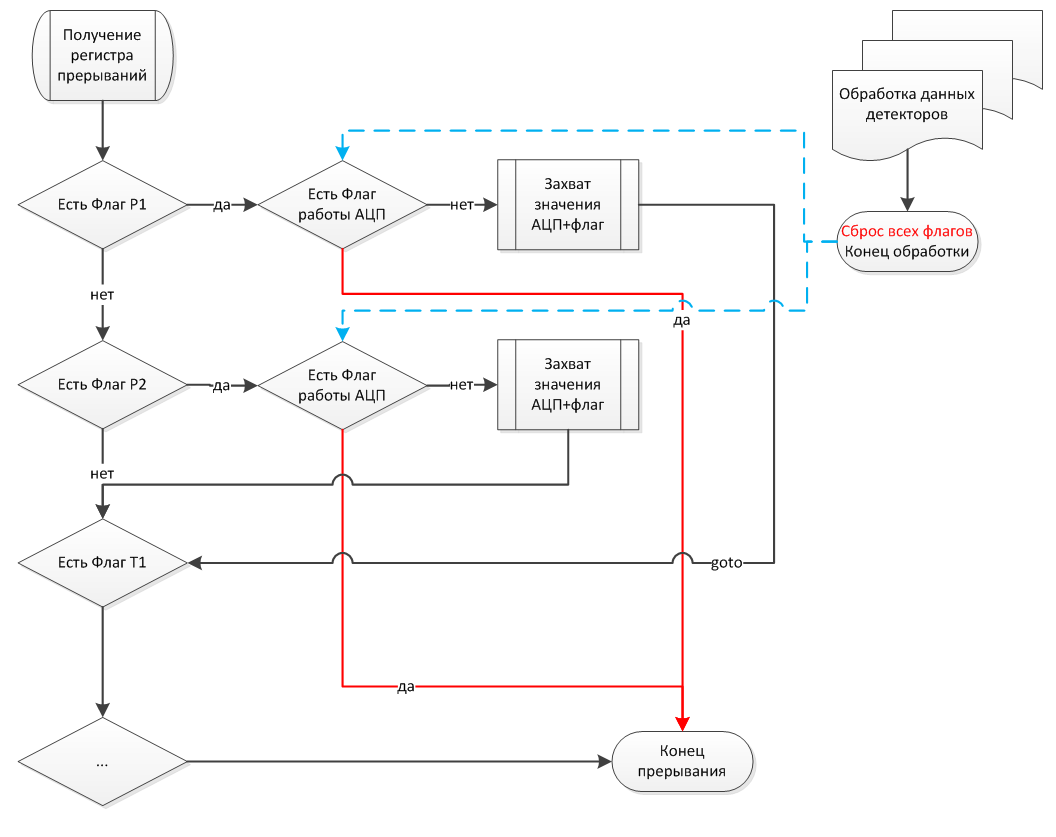
\includegraphics[width=0.7\linewidth]{images/ext_interrupt}
\caption{Блок схема работы процедуры \texttt{Ext\_Interrupt}}
\label{fig:ext_interrupt}
\end{figure}

Внешние прерывания настроены на регистрацию прохождения положительного фронта импульсов. Не подключенные электрически каналы порта ввода-вывода отключены программным образ, подробно подключенные прерывания перечислены в таблице \ref{tab:int}.

\begin{table} 
	\begin{tabular}{|c|c|c|c|}
		\hline
		Номер бита, &  Источник  &       Примечание        &       Описание       \\
		  (PB №)    & прерывания &                         &  \\ \hline
		     4      &  JP2 \# 5  & 1-й нейтронный счетчик  &  \\ \hline
		     5      & JP2 \# 11  & t-сигнал 1-го детектора & верхний п-п детектор \\ \hline
		    10      &  JP2 \# 1  &  Окончание сигнала S1   &  \\ \hline
		    11      &  JP2 \# 7  & 2-й нейтронный счетчик  &  \\ \hline
		    12      &  JP2 \# 9  & t-сигнал 1-го детектора &  аппаратный счетчик  \\ \hline
		    13      & JP2 \# 13  & t-сигнал 2-го детектора & нижний п-п детектор  \\ \hline
		    16      &  JP \# 3   &  Окончание сигнала S2   &   не используется    \\ \hline
	\end{tabular} 
	\caption{Распределение битов в регистре прерывания}
	\label{tab:int}
\end{table}




\subsubsection{Процедура обработки данных с детекторов}

Основная часть программной обработки данных с детекторов прибора производится в процедуре Detectors\_Handling, листинг которой представлен в Приложении \ref{list:Detectors_Handling}.
%\todo{Блок схема работы процедуры Detectors\_Handling}




\subsection{Контрольная проверочная аппаратура}

Контрольно-приемная аппаратура (КПА) прибора ДЭПРОН используется для  проведения автономных испытаний прибора. КПА ДЭПРОН состоит из:


\begin{itemize}
	\item 	Ноутбук (или другой персональный компьютер) с установленной операционной системой Windows XP и установленным специальным программным обеспечением (программой Depron Terminal), наличием порта RS232, либо дополнительно преобразователь интерфейсов USBRS232;
	
	
	\item 	Блока питания, обеспечивающего измерение потребляемого тока нагрузки GwINSTEK GPS-4303;
	
	
	\item 	Преобразователя интерфейсов USBRS232 (при отсутствии COM порта у ПК);
	
	
	\item 	Комплекта соединительных кабелей 
	
	
	\item 	Блока КП -- контрольно-приемного блока
	
	
\end{itemize}





\begin{figure}
	\centering
	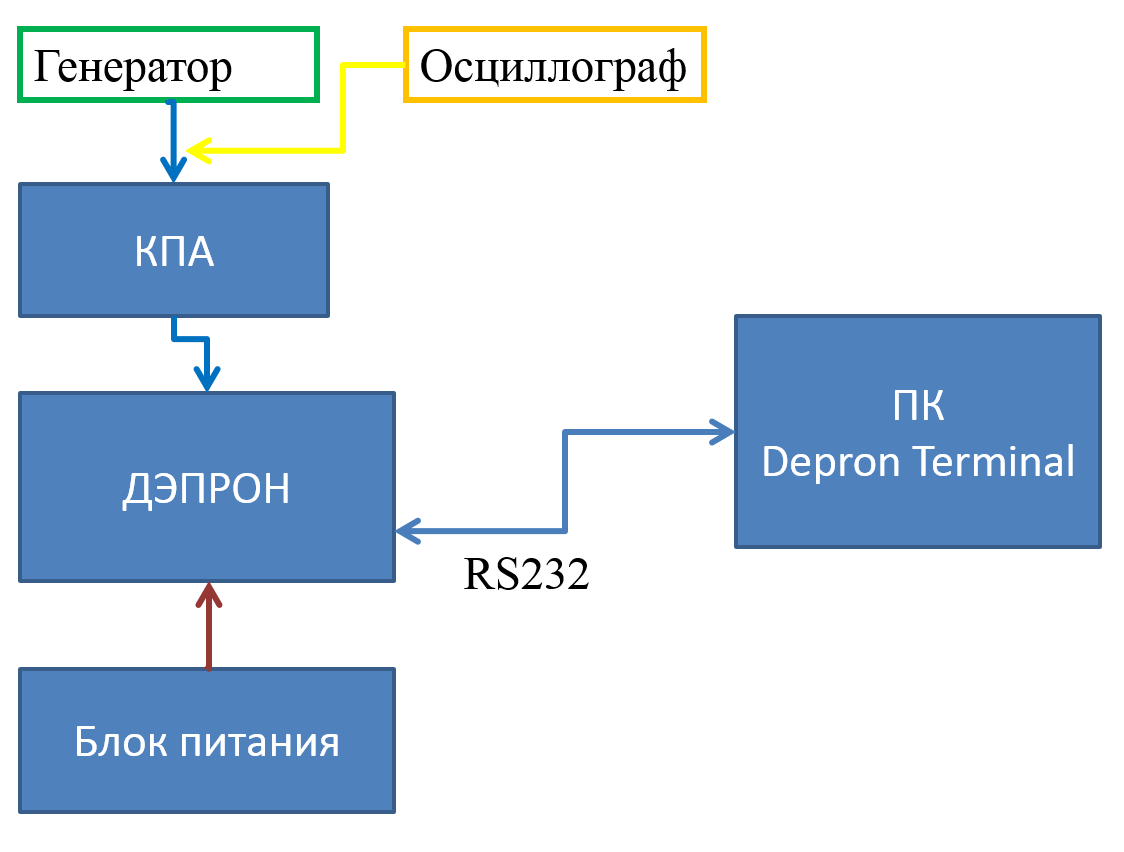
\includegraphics[width=0.49\linewidth]{images/kalibr}
	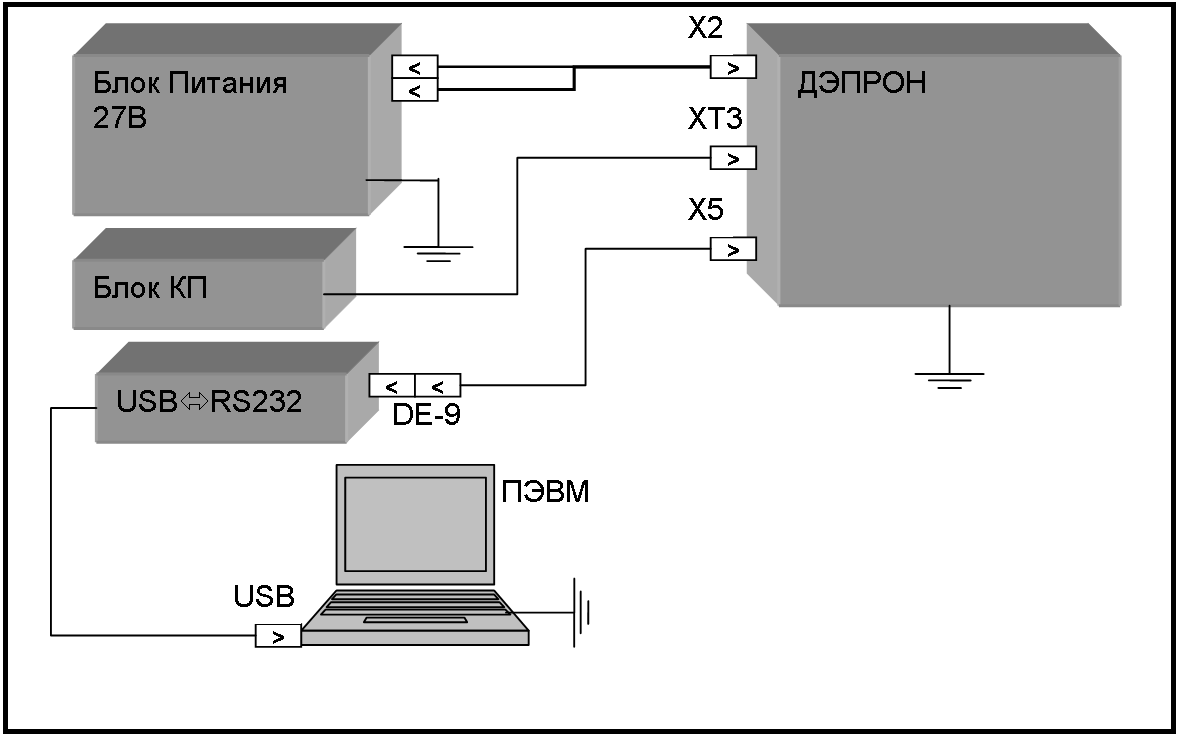
\includegraphics[width=0.49\linewidth]{images/kalibr1}
	\caption[Схема подключения прибора при калибровке]{ Схема подключения КПА для проверки функционирования прибора ДЭПРОН.}
	\label{fig:kalibr}
\end{figure}



Блок КП предназначен для подключения генератора и осциллографа к тестовым входам прибора ДЭПРОН, а также для контроля наличия рабочих напряжений в контурах прибора. Блок КП имеет 4 входных гнезда BNC, маркированные в соответствии с каналами прибора ДЭПРОН на которые передаются тестовые сигналы с генератора X1 и	X2, на первой и второй генераторный выходы. 


На лицевой панели блока КП расположены 2 светодиодных индикатора. Подключение Блока КП к прибору ДЭПРОН происходит через тестовый вход XT3 (типа РС19).


\section{Градуировочные характеристики прибора}
Градуировка прибора ДЭПРОН проводится с использованием известной зависимости 
\ref{eq:benghin_doze_code}

\begin{equation}\label{eq:benghin_doze_code}
D = \frac{E}{m} = \dfrac{w_i \cdot\frac{q}{e}}{m} = \frac{w_i \cdot \Delta U \cdot\sum K \cdot C}{m \cdot e \cdot \eta}  = V \cdot \sum K
\end{equation}
по материалам  «ПРИБОР ДЭПРОН, В.В.~Бенгин, О.Ю.~Нечаев, И.А.~Брильков, А. Ю.~Амелюшкин, В. Л.~Петров»  представленной на рабочем совещании «Universat» (Университетские спутники), 7-10 июня в МГУ им.~М.В.~Ломоносова

где \begin{description}	
	\item[$ K $] выходной сигнал АЦП
	\item[$ C $] входная емкость системы детектор-предусилитель
	\item[$ \eta $] суммарный градуировочный коэффициент тракта усиления до АЦП
	\item[$ \Delta U $] шаг дискретизации АЦП
\end{description} 
Большая часть величин в этой формуле известна, а экспериментально были определены недостающие величины. Данная работа была проведена Сиволаповым Виктором под руководством В.В.~Бенгина \ref{fig:kalibr2}, опираясь на полученные результаты можно провести расчет энергетических коэффициентов для получения величин дозы.

\begin{figure}
	\centering
	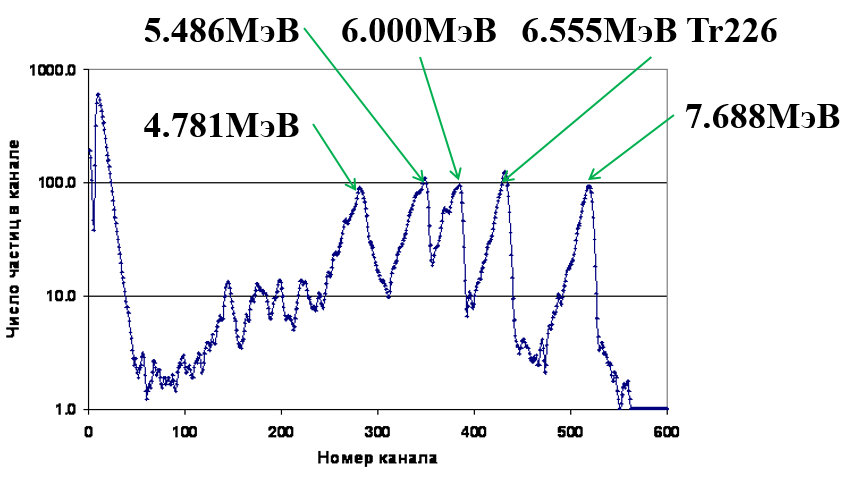
\includegraphics[width=0.49\linewidth]{images/kalibr2}
	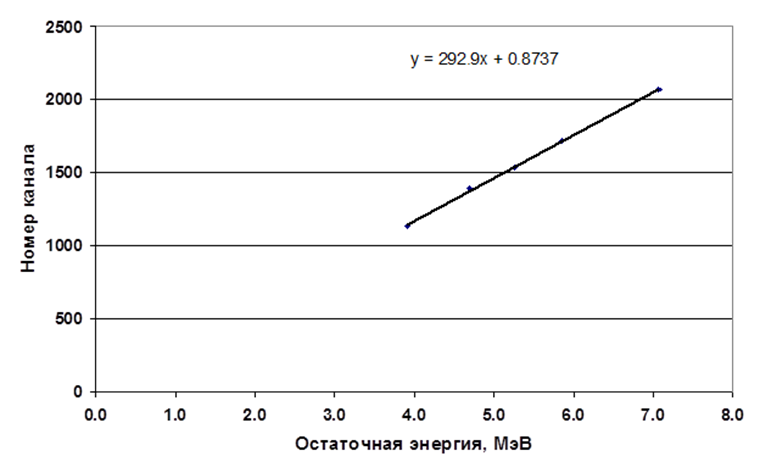
\includegraphics[width=0.49\linewidth]{images/kalibr3}
	\caption[Градуировка прибора на ИИ]{Градуировка прибора на ИИ. Слева спектр энерговыделения для источника Ra-226, отмечены пики соответствующие основным энергетическим линиям Ra и продуктов его распада. Справа показана зависимость энергии альфа-пика от номера канала для значений толщины тормозящего слоя вещества 0.0013~г/см2 (соответствует 5.58~мкм кремния или 1.04~см воздуха).	}
	\label{fig:kalibr2}
\end{figure}
Детектор 1: 3,4141~КэВ/канал 

Детектор 2: 4~КэВ/канал %- очень большой разброс по калибровкам - не могу понять почему:15.4 -- 16.3~КэВ/канал. 

В ходе калибровок получено, что одной единице по дозе детектора 1 соответствует 135 счетных импульсов в детектору 1, таким образом, умножив 135 на 3,4141~кэВ/канал  получаем энергетический эквивалент 3687~кэВ/(дозовый импульс) 

Так как мы имеем квадратный детектор с размерами 10~мм * 10~мм* 300~мкм, оценим массу чувствительного объема детектора, подобрав значения толщины тормозящего слоя вещества $ 0.0013$~г/см$^2$. Такая масса соответствует 5,58~мкм кремния или 1,04 см воздуха, а масса детектора соответственно: 0,0687~г.

Дет1: 8,69~пГр/кодАЦП  0,06952 = 1~нГр/импульс(умноженное на 8)

Дет2: 9,32~пГр/кодАЦП  0,07456 = 1~нГр/импульс(умноженное на 8)


В программе микроконтроллера Дэпрон с целью сокращения передачи не информативных  каналов АЦП был сделан сдвиг на 3 разряда при записи в спектр энерговыделения, такая операция близка к операции деления на 8.

Независимый расчет дал результат для коэффициентов для первого детектора 
0,0633~нГр/импульс, для второго -  0,0742~нГр/импульс. С учетом 
коэффициента 8 это близко к полученным результатам.

\section{Энергетическая чувствительность прибора ДЭПРОН} \label{sec:energy}

В процессе разработки прибор не проходил в полном объеме испытаний на спектральную чувствительность к различным типа излучений, были проведены только калибровки детектирующих узлов на радиоактивных источниках.

Наиболее чувствительный информационный параметр при работе ДЭПРОН --- скорость счета детектора 1. Проведем оценку минимальной энергии заряженных частиц, к которым данный детектор чувствителен. Так как детектор закрыт сверху алюминиевой крышкой толщиной 2~мм, он должен быть чувствителен к протонам с энергией больше 20~МэВ и электронам с энергией больше примерно 0,5~МэВ, а также - возможно - к тормозному излучению. Порог дискриминации сигналов с детектора около 100~КэВ. Тем не менее вопрос уточнения границы чувствительности по минимальным энергиям продолжает оставаться важным и на первом этапе были проведены оценки с помощью данных по проникновению электронов и протонов с сайта NIST \cite{NIST}, физическая модель лежащая в основе этих данных основывается на теории Бете\cite{Bethe1930} с поправкой Штернхаймера \cite{Sternheimer1952} на плотность вещества и подробно описана в ряде статей этого института \cite{Bichsel1992, Ashley1972}.

\begin{figure}[H]
	\centering
	%	\fcolorbox{red}{yellow}{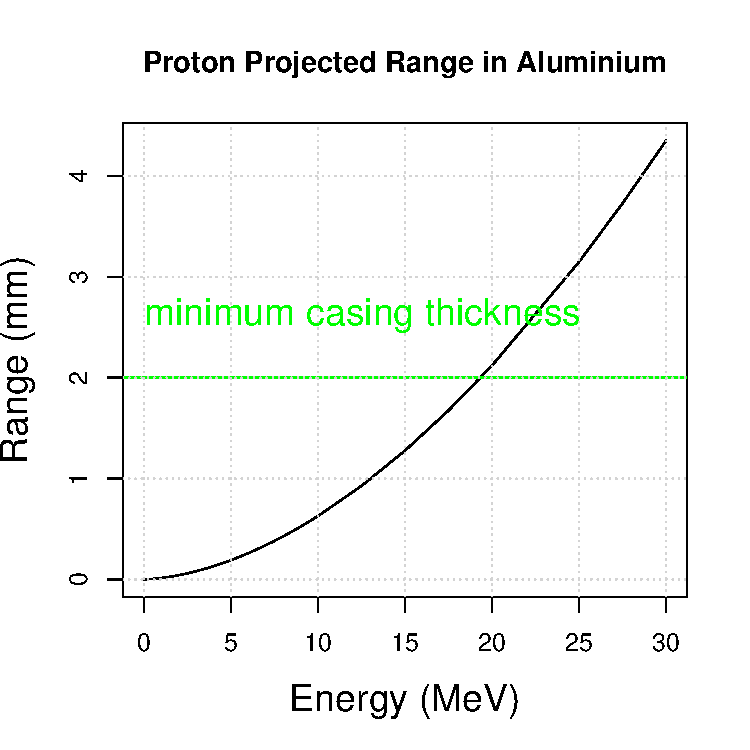
\includegraphics[width=0.6\linewidth]{images/pdata}
%	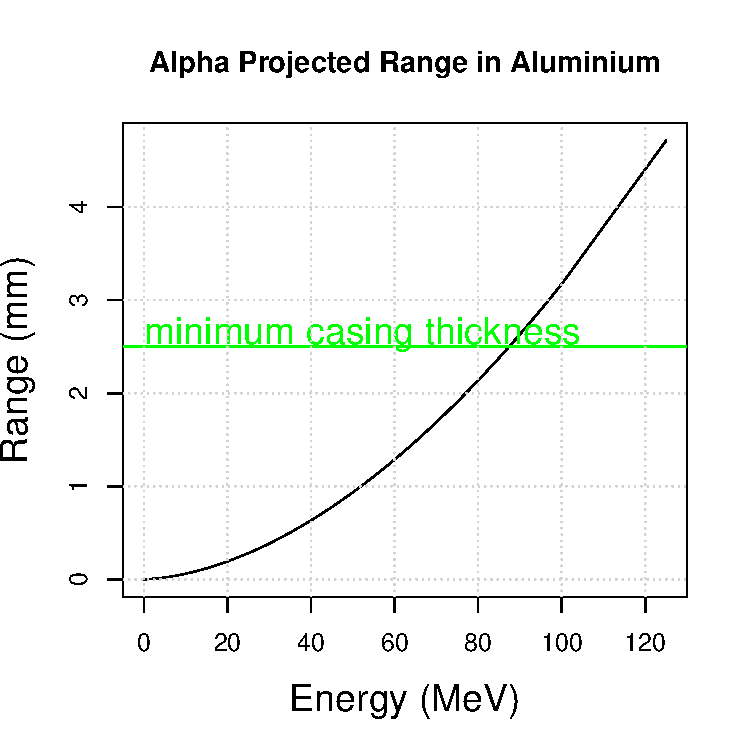
\includegraphics[width=0.6\linewidth]{images/adata}}

	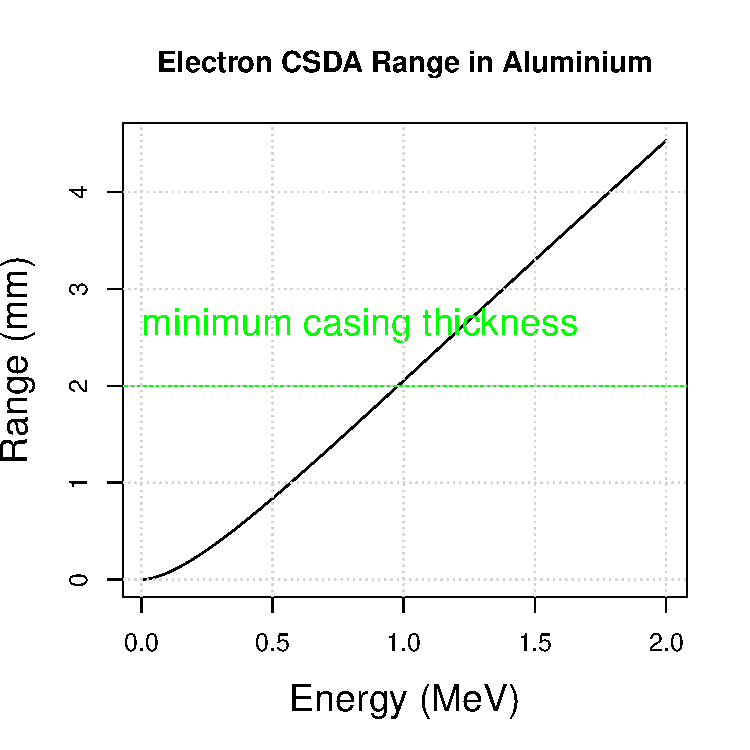
\includegraphics[width=0.32\linewidth]{images/edata}
	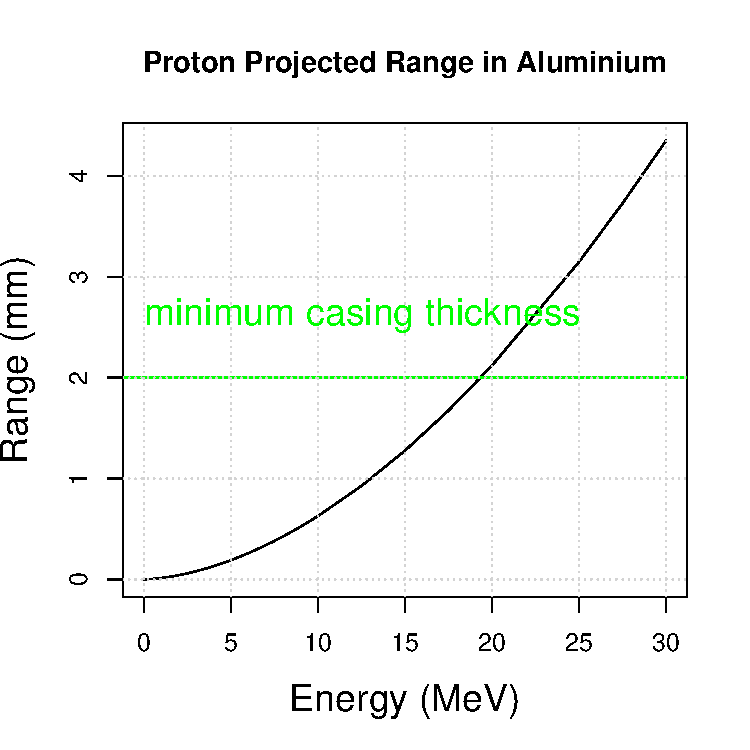
\includegraphics[width=0.32\linewidth]{images/pdata}
	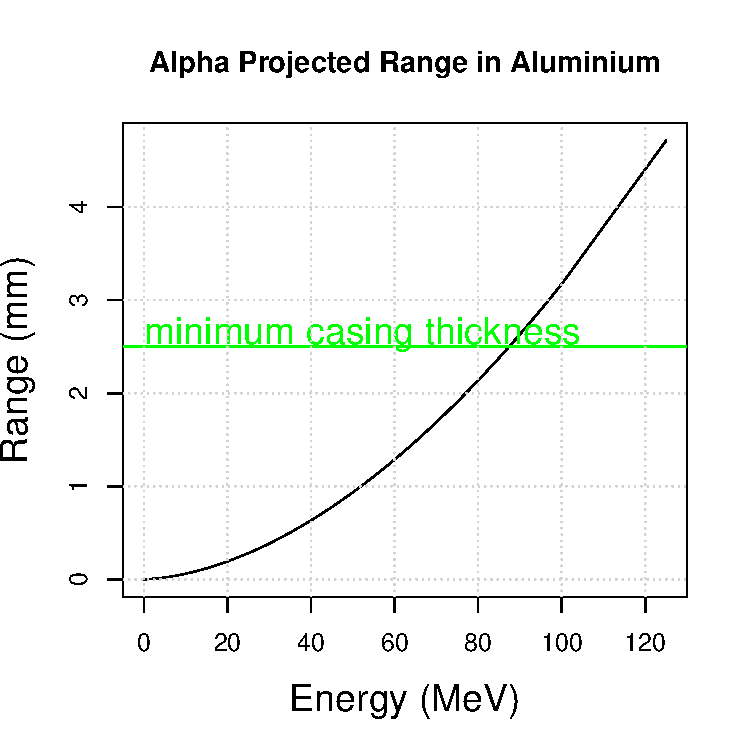
\includegraphics[width=0.32\linewidth]{images/adata}
	\caption{Графики средних пробегов заряженных частиц для алюминия. Представлены величины: ``CSDA range'' --- глубина в приближении непрерывного замедления ``Projected range'' --- среднее значение глубины, на которую заряженная частица проникает в процессе замедления до остановки}
	\label{fig:rplot01}
\end{figure}

Пользуясь представленными зависимостями, для уточненной минимальной толщины корпуса прибора --- она составляет 2,5~мм, что составляет 0,65~г/см\textsuperscript{2}, была повышена предварительная оценка порога нижних энергий, которые способен регистрировать ДЭПРОН по электронам до 1~МэВ и по протонам до 20~МэВ. Для ядер гелия прибор чувствителен начиная с 90~МэВ. Так как эти зависимости могут использоваться только для средних пробегов частиц, для оценки функции энергетической чувствительности требуется более подробный анализ, который может быть произведен с помощью Монте-Карло моделирования.


%\begin{figure}
%	\centering
%	\fcolorbox{red}{yellow}{
%		{\color{green}
%		\stackinset{l}{1in}{b}{1.1in}{\rotatebox{0}{\rule{3.5in}{1pt}}}{%
%			\stackinset{l}{.3in}{b}{}{\rotatebox{85}{\rule{4in}{1pt}}}{%
%				\stackinset{r}{.5in}{b}{}{\rotatebox{-80}{\rule{4in}{1pt}}}{%
%					
%\stackinset{r}{1in}{b}{-.3in}{\rotatebox{-85}{\rule{4in}{1pt}}}{%
%						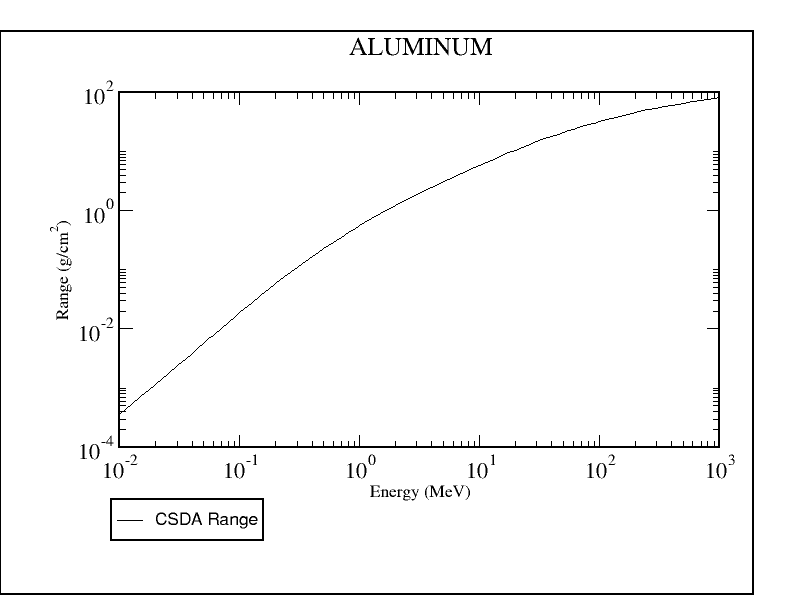
\includegraphics[width=3.5in]{images/graph_elec}
%						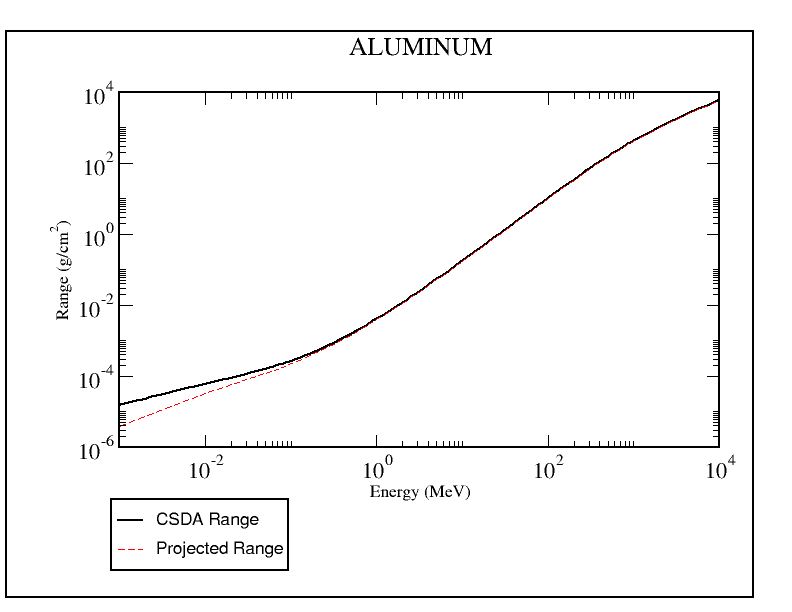
\includegraphics[width=3.5in]{images/graph_prot}
%						
%%%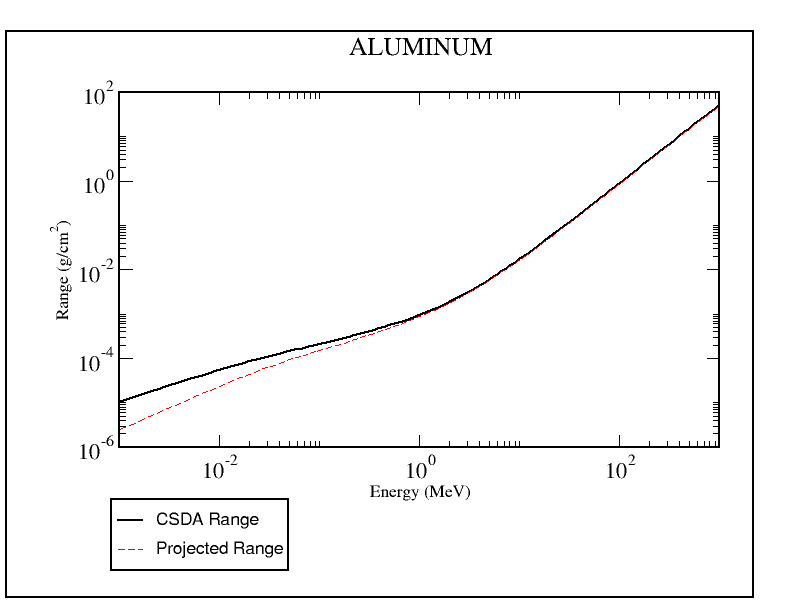
\includegraphics[width=0.7\linewidth]{images/graph_alpha}%
%	}}}}}}
%	\caption{}
%\label{fig:graphelec}
%\end{figure}


\section{Моделирование функций отклика прибора в geant4}

Первично для расчетов прибора Дэпрон использовался FTFP\_BERT так как этот лист предлагается для физики высоких энергий и космической физики. Однако этот список физических явлений очень посредственно описывает поведение тепловых нейтронов и особенно регистрацию в гелиевых счетчиках.
Поэтому для моделирования работы нейтронных детекторов был использован лист физических явлений QGSP\_BIC\_HP \cite{Wright2007}. QGSP~--- основной список физики, использующий кварк-глюонную струнную модель для высокоэнергетических взаимодействий протонов, нейтронов, пионов, каонов и ядер.  Взятый нами физический лист QGSP\_BIC\_HP подобен QGSP, но отличается расчетом бинарного каскада Geant4 для первичных протонов и нейтронов с энергиями ниже \~ 10~ГэВ, таким образом, заменяя использование LEP-модели для протонов и нейтронов. По сравнению с моделью LEP бинарный каскад лучше описывает образование вторичных частиц, образующихся во взаимодействиях Протонов и нейтронов с ядрами. QGSP\_BIC\_HP отличается от QGSP\_BIC добавлением использования базы данных по взаимодействиям нейтронов высокой точности (NeutronHP) для транспортировки нейтронов ниже 20~МэВ и до тепловых энергий. Именно этот список физических явлений рекомендуется для применения в моделировании защиты от радиации и медицинских приложений \cite{Wright2007}.

Для моделирования функционирования нейтронных детекторов необходимо создавать специфический список учитываемых физических явлений по мнению Gregor Simmer\cite{Simmer2007}. Список должен включать упругие и неупругие взаимодействия для нейтронов низких энергий. Выбранный список QGSP\_BIC\_HP соответствует этим требованиям. С полным списком зарегистрированных процессов при моделировании нейтронных счетчиков можно ознакомиться \ref{list:geantNeuproc}.
\begin{figure}
	\centering
	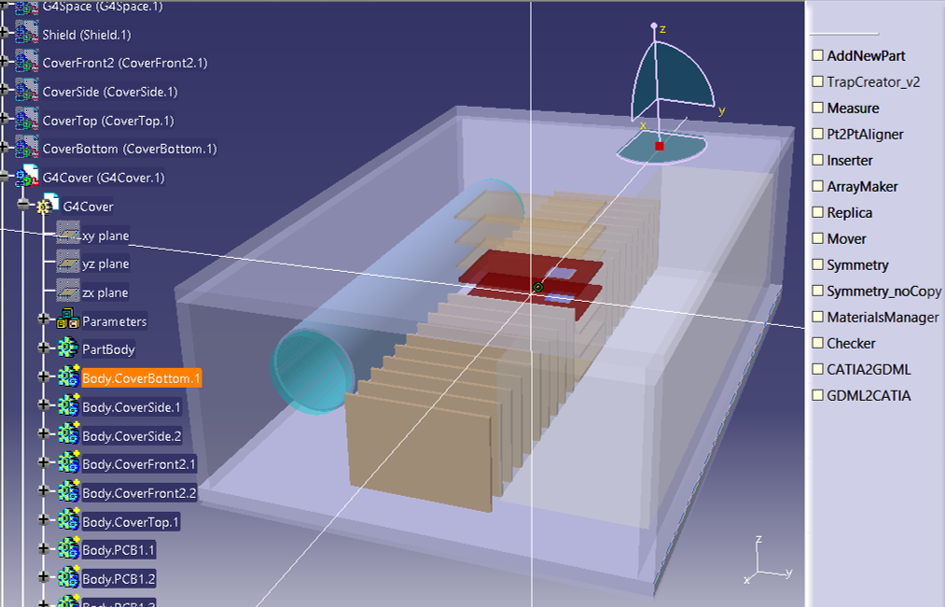
\includegraphics[width=0.49\linewidth]{images/deproncatia2}
	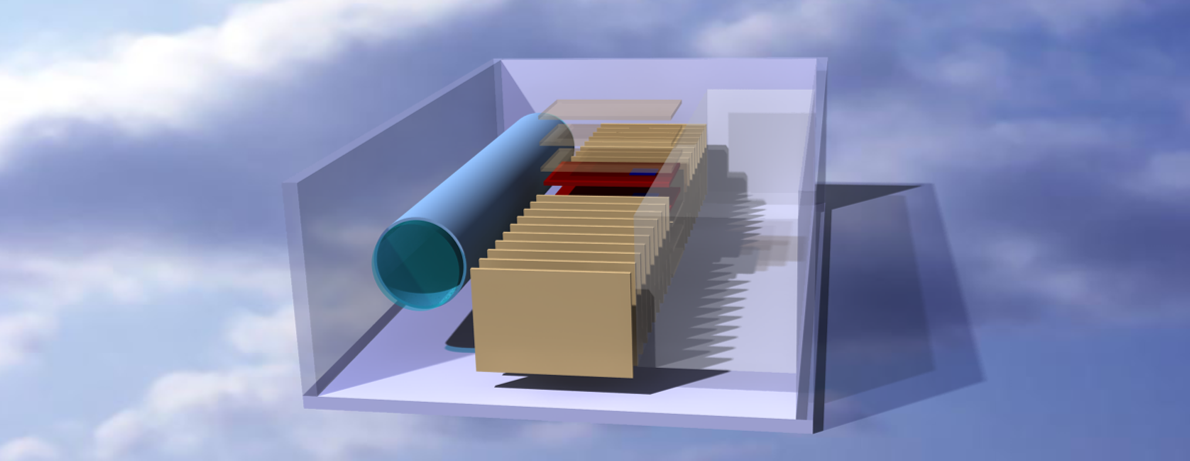
\includegraphics[width=0.49\linewidth]{images/deproncatia}
	\caption[Модель прибора ДЭПРОН]{Подготовка модели прибора в CAD системе. Для наглядности часть деталей, составляющих корпус модели показаны полупрозрачными. }
	\label{fig:deproncatia2}
\end{figure}

С помощью набора макросов ``CATIA-GDML geometry builder''\cite{Belogurov2011a,Belogurov2014} была подготовлена геометрия прибора ДЭПРОН для использования в среде Geant4. Это программное средство значительно упрощает первоначальное построение в CAD системе 3d модели исследуемых приборов на основе комбинации геометрических примитивов. Геометрические примитивы gdml из которых происходит построение модели не являются естественными для CAD Catia, поэтому построение модели целиком производится с помощью макросов, и система проектирования используется для отображения построенной модели и расстановки составляющих объемов \ref{fig:neutron}.


\begin{figure}
	\centering
	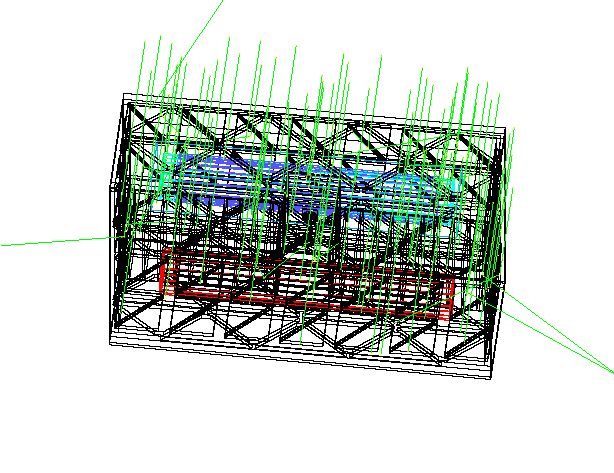
\includegraphics[width=0.7\linewidth]{images/neutrons/neutron}
	\caption[Моделирование работы нейтронных счетчиков в Geant4.]{Моделирование работы нейтронных счетчиков в Geant4. Голубым цветом показан счетчик, окруженный защитой из плексигласа(название чувствительного объема по файлу геометрии si13n1), а красным - счетчик без защиты, si13n2}
	\label{fig:neutron}
\end{figure}

Наиболее важным моментом подготовки модели перед импортом в geant4 является ассоциация каждому объему материала, достаточно точно и полно описывающее атомный состав, и плотность веществ. Опытным путем получено, что большее значение имеет точное описание близлежащих к детекторам материалов и объемов. Однако не следует пренебрегать точностью описания материалов корпуса, так как все частицы РПЗ и ГКЛ вынуждены проходить через стенки прибора. В случае прибора Дэпрон первая версия gdml файла описывала стенки прибора как металлический алюминий, а последующий переход к описанию материала корпуса как дюралюминия привел к значительному увеличению числа вторичных частиц на потоке протонного излучения и гамма излучения, несмотря на то, что количество атомов примесей в сплаве Д16т не превышает 7\%.
Так как гелиевые счетчики заполнены $ ^3\!He $ под давлением в 5 атмосфер, для целей моделирования наполнение счетчиков описано в gdml файле таким образом:
1) Определен He3 как изотоп 
2) Определен элемент He3, состоящий из этого изотопа (100\% He3) 
3) Из элемента определен материал газ He3.

Тестовый источник излучения для проверки чувствительности нейтронных детекторов был представлен как набор последовательных монохроматических линий нейтронного излучения с плоскости на расстоянии 10~см от верхней крышки прибора. Шаг по энергии между соседними линиями подобран чтобы на каждый порядок приходилось по 3 монолинии.  
Итоговая схема моделирования 27 линий с $ 10^5 $ нейтронов в каждом пакете потребовала 32 минут процессорного времени на виртуальной машине geant4.9.6 с 4-мя ядрами Intel i7 3,4 ГГц.
\begin{figure}
	\centering
	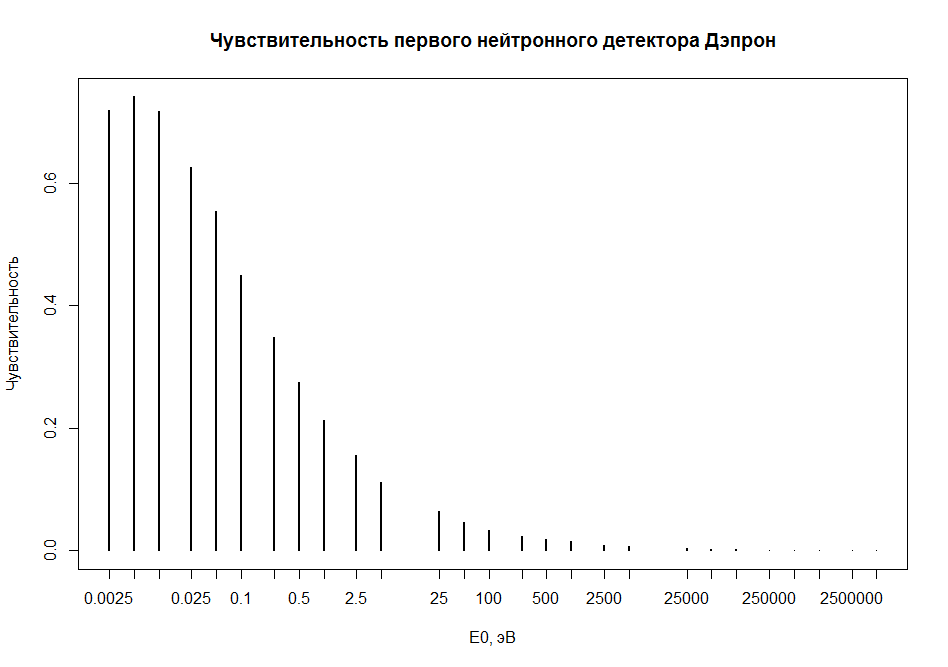
\includegraphics[width=0.6\linewidth]{images/neutrons/nsens1}
	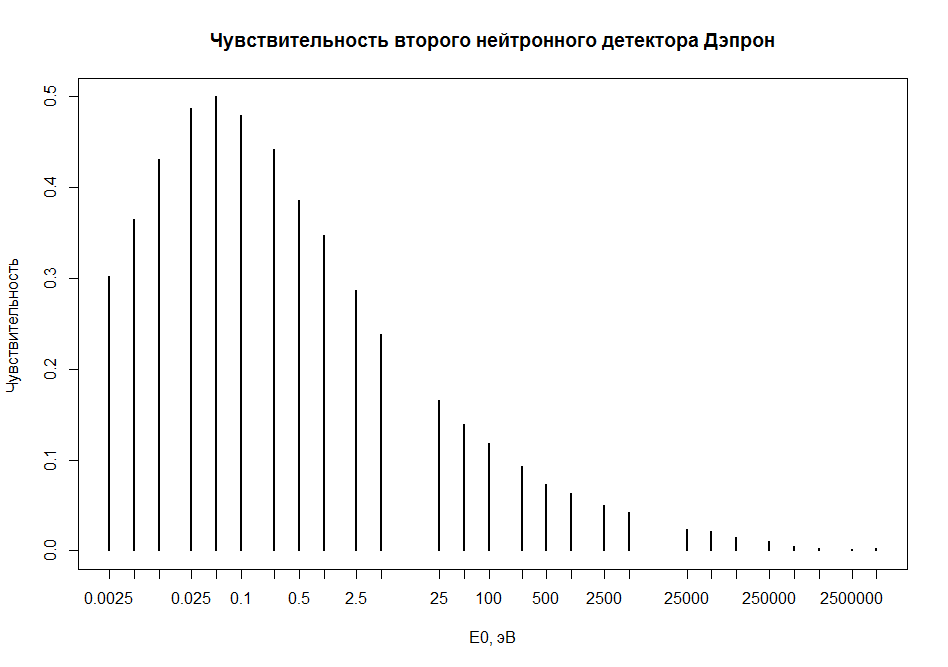
\includegraphics[width=0.6\linewidth]{images/neutrons/nsens2}
	\caption{Профили чувствительности нейтронных счетчиков по итогам моделирования прибора Дэпрон. }
	\label{fig:nsens1}
\end{figure}
На рисунке \ref{fig:nsens1} показаны гистограммы, отражающие отношение зарегистрированных в счетчиках нейтронов к потоку нейтронов, прошедших через тело счетчика. По определению \ref{eq:sens} эта величина соответствует функции чувствительности. Фактом регистрации нейтрона в детекторе при моделировании считалось энерговыделение в объеме заполняющего газа более 500~кэВ. При сравнении профилей чувствительности не защищенного и окруженного оргстеклом нейтронных детекторов можно заметить что пик чувствительности более защищенного детектора находится на 0,005~эВ, а для защищенного этот пик находится на 0,5~эВ энергии нейтронов.

Для энергий нейтронов в десятки эВ чувствительность защищенного детектора превышает незащищенный в несколько раз (более, чем в 4 раза). Таким образом на основании данных о сравнительном счете в детекторах прибора можно делать предположения о сравнительном соотношении нейтронов различных энергий в общем потоке.
\begin{figure}
	\centering
	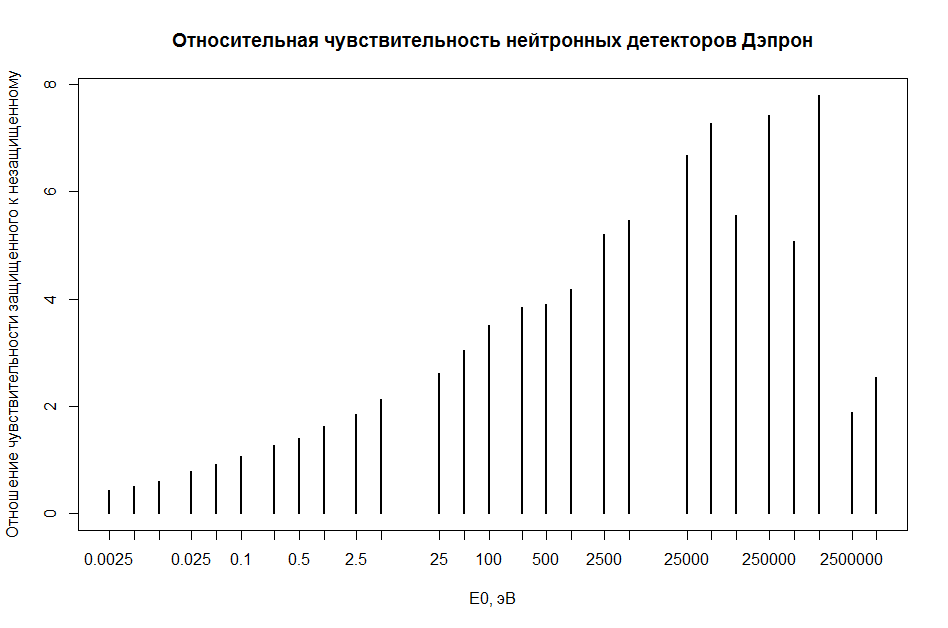
\includegraphics[width=0.6\linewidth]{images/neutrons/otnsensetiv}
	\caption{Оценка относительной чувствительности нейтронных детекторов при различных энергиях нейтронов.}
	\label{fig:otnsensetiv}
\end{figure}



